\section{Scope and recorded coverage}
Board PM12-\allowbreak{}K7-\allowbreak{}3A17A1\allowbreak{}B40221\allowbreak{}2223. Campaign 5ef2e2\allowbreak{}b4-\allowbreak{}c04a-\allowbreak{}4fad-\allowbreak{}b86f-\allowbreak{}a23be6\allowbreak{}21d7a7\allowbreak{}.

Recorded status: INCOMP\allowbreak{}LETE. Missing tests are NOT MEASURED. Complete selected-protocol coverage is not a calibrated whole-board release.

\begingroup\setlength{\tabcolsep}{3pt}\begin{longtable}{>{\raggedright\arraybackslash}p{0.1075\linewidth}>{\raggedright\arraybackslash}p{0.1075\linewidth}>{\raggedright\arraybackslash}p{0.1075\linewidth}>{\raggedright\arraybackslash}p{0.1075\linewidth}>{\raggedright\arraybackslash}p{0.1075\linewidth}>{\raggedright\arraybackslash}p{0.1075\linewidth}>{\raggedright\arraybackslash}p{0.1075\linewidth}>{\raggedright\arraybackslash}p{0.1075\linewidth}}\toprule
Channe\allowbreak{}l & cfd-\allowbreak{}monito\allowbreak{}r & cfd-\allowbreak{}dacs & gate-\allowbreak{}phase & tdc & adc-\allowbreak{}dc & adc-\allowbreak{}lines & integr\allowbreak{}ator\\\midrule\endhead
1 & NM & NM & NM & NM & NM & NM & NM\\
2 & NM & NM & NM & NM & NM & NM & NM\\
3 & NM & NM & NM & NM & NM & NM & NM\\
4 & NM & NM & NM & NM & NM & NM & NM\\
5 & NM & NM & NM & NM & NM & NM & NM\\
6 & NM & NM & NM & NM & NM & NM & NM\\
7 & NM & NM & NM & NM & NM & NM & NM\\
8 & NM & NM & NM & NM & NM & NM & NM\\
9 & NM & PASS & NM & NM & NM & NM & NM\\
10 & NM & PASS & NM & NM & NM & NM & NM\\
11 & NM & PASS & NM & NM & NM & NM & NM\\
12 & NM & PASS & NM & NM & PASS & PASS & PASS\\
\bottomrule\end{longtable}\endgroup
NM = not measured; INC = incomplete; ERR = acquisition error. No missing series is invented.
\subsection{Board-level tests}
\begingroup\setlength{\tabcolsep}{3pt}\begin{longtable}{>{\raggedright\arraybackslash}p{0.4300\linewidth}>{\raggedright\arraybackslash}p{0.4300\linewidth}}\toprule
Test & Status\allowbreak{}\\\midrule\endhead
Bounda\allowbreak{}ry scan and CPLD–FPGA connec\allowbreak{}tions & NOT\_\allowbreak{}MEASUR\allowbreak{}ED\\
MCU,\allowbreak{} CPU–FPGA commun\allowbreak{}icatio\allowbreak{}n and periph\allowbreak{}eral IDs & NOT\_\allowbreak{}MEASUR\allowbreak{}ED\\
I2C sensor\allowbreak{}s,\allowbreak{} curren\allowbreak{}ts and voltag\allowbreak{}es & NOT\_\allowbreak{}MEASUR\allowbreak{}ED\\
HDMI digita\allowbreak{}l link & NOT\_\allowbreak{}MEASUR\allowbreak{}ED\\
Ethern\allowbreak{}et/\allowbreak{}bridge\allowbreak{} diagno\allowbreak{}stic & NOT\_\allowbreak{}MEASUR\allowbreak{}ED\\
\bottomrule\end{longtable}\endgroup
\section{Fitted batches and fixture provenance}
\begingroup\setlength{\tabcolsep}{3pt}\begin{longtable}{>{\raggedright\arraybackslash}p{0.1720\linewidth}>{\raggedright\arraybackslash}p{0.1720\linewidth}>{\raggedright\arraybackslash}p{0.1720\linewidth}>{\raggedright\arraybackslash}p{0.1720\linewidth}>{\raggedright\arraybackslash}p{0.1720\linewidth}}\toprule
Batch attemp\allowbreak{}t & PM channe\allowbreak{}l & CFD label & Declar\allowbreak{}ed connec\allowbreak{}tion & Fittin\allowbreak{}g\\\midrule\endhead
ch09-\allowbreak{}12-\allowbreak{}attemp\allowbreak{}t001 & 12 & CFD01 & slot 7,\allowbreak{} RJ45 0 & Identi\allowbreak{}ty/\allowbreak{}fittin\allowbreak{}g confir\allowbreak{}med\\
ch09-\allowbreak{}12-\allowbreak{}attemp\allowbreak{}t001 & 11 & CFD02 & slot 7,\allowbreak{} RJ45 1 & Identi\allowbreak{}ty/\allowbreak{}fittin\allowbreak{}g confir\allowbreak{}med\\
ch09-\allowbreak{}12-\allowbreak{}attemp\allowbreak{}t001 & 10 & CFD03 & slot 7,\allowbreak{} RJ45 2 & Identi\allowbreak{}ty/\allowbreak{}fittin\allowbreak{}g confir\allowbreak{}med\\
ch09-\allowbreak{}12-\allowbreak{}attemp\allowbreak{}t001 & 9 & CFD04 & slot 7,\allowbreak{} RJ45 3 & Identi\allowbreak{}ty/\allowbreak{}fittin\allowbreak{}g confir\allowbreak{}med\\
\bottomrule\end{longtable}\endgroup
Fixture labels CFD01--CFD04 are provisional bench labels. Factory identities and photos remain unknown until supplied; a label is not proof of module identity. Declared cable routes must be checked physically.

Raw inputs and selected result IDs are retained in inputs/. Repeated measurements are never silently substituted.
\section{Retained attempts and explicit selection}
\begingroup\setlength{\tabcolsep}{3pt}\begin{longtable}{>{\raggedright\arraybackslash}p{0.1433\linewidth}>{\raggedright\arraybackslash}p{0.1433\linewidth}>{\raggedright\arraybackslash}p{0.1433\linewidth}>{\raggedright\arraybackslash}p{0.1433\linewidth}>{\raggedright\arraybackslash}p{0.1433\linewidth}>{\raggedright\arraybackslash}p{0.1433\linewidth}}\toprule
Result\allowbreak{} ID prefix\allowbreak{} & Test & Channe\allowbreak{}l & Fittin\allowbreak{}g & Status\allowbreak{} & Select\allowbreak{}ed\\\midrule\endhead
result\allowbreak{}-\allowbreak{}b91262\allowbreak{}35 & adc-\allowbreak{}dc & 12 & ch09-\allowbreak{}12-\allowbreak{}attemp\allowbreak{}t001 & PASS & yes\\
result\allowbreak{}-\allowbreak{}ee0613\allowbreak{}ea & adc-\allowbreak{}lines & 12 & ch09-\allowbreak{}12-\allowbreak{}attemp\allowbreak{}t001 & PASS & yes\\
result\allowbreak{}-\allowbreak{}217f5c\allowbreak{}b4 & integr\allowbreak{}ator & 12 & ch09-\allowbreak{}12-\allowbreak{}attemp\allowbreak{}t001 & PASS & yes\\
result\allowbreak{}-\allowbreak{}b99efe\allowbreak{}3a & cfd-\allowbreak{}dacs & 9 & ch09-\allowbreak{}12-\allowbreak{}attemp\allowbreak{}t001 & INCOMP\allowbreak{}LETE & no\\
result\allowbreak{}-\allowbreak{}ef5049\allowbreak{}3e & cfd-\allowbreak{}dacs & 10 & ch09-\allowbreak{}12-\allowbreak{}attemp\allowbreak{}t001 & INCOMP\allowbreak{}LETE & no\\
result\allowbreak{}-\allowbreak{}c4800a\allowbreak{}66 & cfd-\allowbreak{}dacs & 11 & ch09-\allowbreak{}12-\allowbreak{}attemp\allowbreak{}t001 & INCOMP\allowbreak{}LETE & no\\
result\allowbreak{}-\allowbreak{}c80f3b\allowbreak{}9e & cfd-\allowbreak{}dacs & 12 & ch09-\allowbreak{}12-\allowbreak{}attemp\allowbreak{}t001 & INCOMP\allowbreak{}LETE & no\\
result\allowbreak{}-\allowbreak{}9e64b4\allowbreak{}3e & cfd-\allowbreak{}dacs & 9 & ch09-\allowbreak{}12-\allowbreak{}attemp\allowbreak{}t001 & PASS & yes\\
result\allowbreak{}-\allowbreak{}0fcaad\allowbreak{}d7 & cfd-\allowbreak{}dacs & 10 & ch09-\allowbreak{}12-\allowbreak{}attemp\allowbreak{}t001 & PASS & yes\\
result\allowbreak{}-\allowbreak{}8b6b8a\allowbreak{}a7 & cfd-\allowbreak{}dacs & 11 & ch09-\allowbreak{}12-\allowbreak{}attemp\allowbreak{}t001 & PASS & yes\\
result\allowbreak{}-\allowbreak{}b4c6c4\allowbreak{}97 & cfd-\allowbreak{}dacs & 12 & ch09-\allowbreak{}12-\allowbreak{}attemp\allowbreak{}t001 & PASS & yes\\
\bottomrule\end{longtable}\endgroup
All attempts, including failures and rejected repeats, remain in the archived inputs. The coverage matrix uses only the explicitly selected attempt.
\section{Selected measurement conditions and limits}
\begingroup\setlength{\tabcolsep}{3pt}\begin{longtable}{>{\raggedright\arraybackslash}p{0.2867\linewidth}>{\raggedright\arraybackslash}p{0.2867\linewidth}>{\raggedright\arraybackslash}p{0.2867\linewidth}}\toprule
Test & Physic\allowbreak{}al channe\allowbreak{}l & Confir\allowbreak{}med stimul\allowbreak{}us connec\allowbreak{}tion\\\midrule\endhead
adc-\allowbreak{}dc & 12 & \{"dac\_\allowbreak{}channe\allowbreak{}ls": [0,\allowbreak{} 1],\allowbreak{} "stimul\allowbreak{}us\_\allowbreak{}channe\allowbreak{}l": 12,\allowbreak{} "usb\_\allowbreak{}input": "J8"\}\\
adc-\allowbreak{}lines & 12 & \{"dac\_\allowbreak{}channe\allowbreak{}ls": [0,\allowbreak{} 1],\allowbreak{} "stimul\allowbreak{}us\_\allowbreak{}channe\allowbreak{}l": 12,\allowbreak{} "usb\_\allowbreak{}input": "J8"\}\\
integr\allowbreak{}ator & 12 & \{"dac\_\allowbreak{}channe\allowbreak{}ls": [2,\allowbreak{} 3],\allowbreak{} "stimul\allowbreak{}us\_\allowbreak{}channe\allowbreak{}l": 12,\allowbreak{} "usb\_\allowbreak{}input": "J6"\}\\
cfd-\allowbreak{}dacs & 9 & \{"select\allowbreak{}ion": "one monito\allowbreak{}r mux enable\allowbreak{}d; all others\allowbreak{} inhibi\allowbreak{}ted",\allowbreak{} "shared\allowbreak{}\_\allowbreak{}monito\allowbreak{}r\_\allowbreak{}channe\allowbreak{}ls": [9,\allowbreak{} 10,\allowbreak{} 11,\allowbreak{} 12]\}\\
cfd-\allowbreak{}dacs & 10 & \{"select\allowbreak{}ion": "one monito\allowbreak{}r mux enable\allowbreak{}d; all others\allowbreak{} inhibi\allowbreak{}ted",\allowbreak{} "shared\allowbreak{}\_\allowbreak{}monito\allowbreak{}r\_\allowbreak{}channe\allowbreak{}ls": [9,\allowbreak{} 10,\allowbreak{} 11,\allowbreak{} 12]\}\\
cfd-\allowbreak{}dacs & 11 & \{"select\allowbreak{}ion": "one monito\allowbreak{}r mux enable\allowbreak{}d; all others\allowbreak{} inhibi\allowbreak{}ted",\allowbreak{} "shared\allowbreak{}\_\allowbreak{}monito\allowbreak{}r\_\allowbreak{}channe\allowbreak{}ls": [9,\allowbreak{} 10,\allowbreak{} 11,\allowbreak{} 12]\}\\
cfd-\allowbreak{}dacs & 12 & \{"select\allowbreak{}ion": "one monito\allowbreak{}r mux enable\allowbreak{}d; all others\allowbreak{} inhibi\allowbreak{}ted",\allowbreak{} "shared\allowbreak{}\_\allowbreak{}monito\allowbreak{}r\_\allowbreak{}channe\allowbreak{}ls": [9,\allowbreak{} 10,\allowbreak{} 11,\allowbreak{} 12]\}\\
\bottomrule\end{longtable}\endgroup
\subsection{Common hardware configuration}
\begingroup\setlength{\tabcolsep}{3pt}\begin{longtable}{>{\raggedright\arraybackslash}p{0.4300\linewidth}>{\raggedright\arraybackslash}p{0.4300\linewidth}}\toprule
Settin\allowbreak{}g & Record\allowbreak{}ed value\\\midrule\endhead
clock\_\allowbreak{}profil\allowbreak{}e.adc\_\allowbreak{}rate & 2x refere\allowbreak{}nce\\
clock\_\allowbreak{}profil\allowbreak{}e.kasli\_\allowbreak{}rate & 3x refere\allowbreak{}nce\\
clock\_\allowbreak{}profil\allowbreak{}e.refere\allowbreak{}nce\_\allowbreak{}mhz & 40.0787\\
cpld\_\allowbreak{}gate\_\allowbreak{}mode & origin\allowbreak{}al INTA/\allowbreak{}INTB enable\allowbreak{}d,\allowbreak{} nomina\allowbreak{}l20MHz\allowbreak{}\\
kasli\_\allowbreak{}build.ABI & CFD4\\
kasli\_\allowbreak{}build.expect\allowbreak{}ed\_\allowbreak{}bit\_\allowbreak{}sha256\allowbreak{} & a71a08\allowbreak{}a25862\allowbreak{}0b0e5a\allowbreak{}52c5d0\allowbreak{}3aefd8\allowbreak{}c69040\allowbreak{}c9d15e\allowbreak{}8de639\allowbreak{}1c484a\allowbreak{}c182b7\allowbreak{}173b\\
pm\_\allowbreak{}build & c7c42d\allowbreak{}28\\
\bottomrule\end{longtable}\endgroup
\subsection{adc-\allowbreak{}dc}
\begingroup\setlength{\tabcolsep}{3pt}\begin{longtable}{>{\raggedright\arraybackslash}p{0.4300\linewidth}>{\raggedright\arraybackslash}p{0.4300\linewidth}}\toprule
Settin\allowbreak{}g & Record\allowbreak{}ed value\\\midrule\endhead
method\allowbreak{} & "direct\allowbreak{}-\allowbreak{}ADC-\allowbreak{}DC-\allowbreak{}v1"\\
stimul\allowbreak{}us\_\allowbreak{}points\allowbreak{}\_\allowbreak{}per\_\allowbreak{}bank & 257\\
comman\allowbreak{}ded\_\allowbreak{}range\_\allowbreak{}V & [-\allowbreak{}1.2,\allowbreak{} 1.2]\\
common\allowbreak{}\_\allowbreak{}mode\_\allowbreak{}V & 1.0\\
dac\_\allowbreak{}channe\allowbreak{}ls & [0,\allowbreak{} 1]\\
fit\_\allowbreak{}interv\allowbreak{}al\_\allowbreak{}V & [-\allowbreak{}0.8,\allowbreak{} 0.8]\\
fft\_\allowbreak{}sample\allowbreak{}\_\allowbreak{}rate\_\allowbreak{}assume\allowbreak{}d\_\allowbreak{}Hz & 801574\allowbreak{}00\\
integr\allowbreak{}ator\_\allowbreak{}input\_\allowbreak{}parked\allowbreak{}\_\allowbreak{}V & [2.048000\allowbreak{}1,\allowbreak{} 1.024000\allowbreak{}05]\\
\bottomrule\end{longtable}\endgroup
\subsection{adc-\allowbreak{}lines}
\begingroup\setlength{\tabcolsep}{3pt}\begin{longtable}{>{\raggedright\arraybackslash}p{0.4300\linewidth}>{\raggedright\arraybackslash}p{0.4300\linewidth}}\toprule
Settin\allowbreak{}g & Record\allowbreak{}ed value\\\midrule\endhead
method\allowbreak{} & "adjace\allowbreak{}nt-\allowbreak{}pair-\allowbreak{}states\allowbreak{}-\allowbreak{}v1"\\
stimul\allowbreak{}us\_\allowbreak{}points\allowbreak{}\_\allowbreak{}per\_\allowbreak{}bank & 257\\
comman\allowbreak{}ded\_\allowbreak{}range\_\allowbreak{}V & [-\allowbreak{}1.2,\allowbreak{} 1.2]\\
common\allowbreak{}\_\allowbreak{}mode\_\allowbreak{}V & 1.0\\
dac\_\allowbreak{}channe\allowbreak{}ls & [0,\allowbreak{} 1]\\
fit\_\allowbreak{}interv\allowbreak{}al\_\allowbreak{}V & [-\allowbreak{}0.8,\allowbreak{} 0.8]\\
fft\_\allowbreak{}sample\allowbreak{}\_\allowbreak{}rate\_\allowbreak{}assume\allowbreak{}d\_\allowbreak{}Hz & 801574\allowbreak{}00\\
integr\allowbreak{}ator\_\allowbreak{}input\_\allowbreak{}parked\allowbreak{}\_\allowbreak{}V & [2.048000\allowbreak{}1,\allowbreak{} 1.024000\allowbreak{}05]\\
\bottomrule\end{longtable}\endgroup
\subsection{cfd-\allowbreak{}dacs}
\begingroup\setlength{\tabcolsep}{3pt}\begin{longtable}{>{\raggedright\arraybackslash}p{0.4300\linewidth}>{\raggedright\arraybackslash}p{0.4300\linewidth}}\toprule
Settin\allowbreak{}g & Record\allowbreak{}ed value\\\midrule\endhead
method\allowbreak{} & "shared\allowbreak{}-\allowbreak{}monito\allowbreak{}r-\allowbreak{}SMU-\allowbreak{}BCD-\allowbreak{}v1"\\
instru\allowbreak{}ment\_\allowbreak{}identi\allowbreak{}ty & "Keysig\allowbreak{}ht Techno\allowbreak{}logies\allowbreak{},\allowbreak{}B2910B\allowbreak{}L,\allowbreak{}MY6332\allowbreak{}0299,\allowbreak{}5.0.2429.8966"\\
sense & "Force HI/\allowbreak{}LO,\allowbreak{} local"\\
source\allowbreak{}\_\allowbreak{}curren\allowbreak{}t\_\allowbreak{}A & 0\\
source\allowbreak{}\_\allowbreak{}range\_\allowbreak{}A & 1e-\allowbreak{}06\\
voltag\allowbreak{}e\_\allowbreak{}range\_\allowbreak{}V & 20\\
nplc & 1\\
settli\allowbreak{}ng\_\allowbreak{}s & 0.1\\
points\allowbreak{} & 101\\
repeat\allowbreak{}s & 3\\
limits\allowbreak{} & \{"repeat\allowbreak{}\_\allowbreak{}std\_\allowbreak{}V": 0.001,\allowbreak{} "revers\allowbreak{}e\_\allowbreak{}step\_\allowbreak{}V": 0.0002,\allowbreak{} "span\_\allowbreak{}relati\allowbreak{}ve\_\allowbreak{}error": 0.05\}\\
post\_\allowbreak{}scan\_\allowbreak{}verifi\allowbreak{}cation\allowbreak{} & "SMU OFF/\allowbreak{}HIZ,\allowbreak{} four monito\allowbreak{}r muxes inhibi\allowbreak{}ted,\allowbreak{} explic\allowbreak{}it TCA masks0\allowbreak{}"\\
\bottomrule\end{longtable}\endgroup
\subsection{integr\allowbreak{}ator}
\begingroup\setlength{\tabcolsep}{3pt}\begin{longtable}{>{\raggedright\arraybackslash}p{0.4300\linewidth}>{\raggedright\arraybackslash}p{0.4300\linewidth}}\toprule
Settin\allowbreak{}g & Record\allowbreak{}ed value\\\midrule\endhead
method\allowbreak{} & "signed\allowbreak{}-\allowbreak{}integr\allowbreak{}ation-\allowbreak{}pair-\allowbreak{}v1"\\
dac\_\allowbreak{}channe\allowbreak{}ls & [2,\allowbreak{} 3]\\
base\_\allowbreak{}V & [1.024,\allowbreak{} 2.048]\\
coarse\allowbreak{}\_\allowbreak{}offset\allowbreak{}s\_\allowbreak{}V & [-\allowbreak{}0.099999\allowbreak{}999999\allowbreak{}99987,\allowbreak{} -\allowbreak{}0.080000\allowbreak{}000000\allowbreak{}00007,\allowbreak{} -\allowbreak{}0.059999\allowbreak{}999999\allowbreak{}99983,\allowbreak{} -\allowbreak{}0.040000\allowbreak{}000000\allowbreak{}000036\allowbreak{},\allowbreak{} -\allowbreak{}0.019999\allowbreak{}999999\allowbreak{}999796\allowbreak{},\allowbreak{} -\allowbreak{}0.010000\allowbreak{}000000\allowbreak{}000009\allowbreak{},\allowbreak{} 0.0,\allowbreak{} 0.009999\allowbreak{}999999\allowbreak{}999787\allowbreak{},\allowbreak{} 0.020000\allowbreak{}000000\allowbreak{}00024,\allowbreak{} 0.040000\allowbreak{}000000\allowbreak{}000036\allowbreak{},\allowbreak{} 0.060000\allowbreak{}000000\allowbreak{}000275\allowbreak{},\allowbreak{} 0.080000\allowbreak{}000000\allowbreak{}00007,\allowbreak{} 0.100000\allowbreak{}000000\allowbreak{}00009]\\
fine\_\allowbreak{}method\allowbreak{} & "26 points\allowbreak{},\allowbreak{}0.4mV step around\allowbreak{} coarse\allowbreak{} estima\allowbreak{}te"\\
return\allowbreak{}\_\allowbreak{}method\allowbreak{} & "two candid\allowbreak{}ate revisi\allowbreak{}ts and +/\allowbreak{}-\allowbreak{}5mV offset\allowbreak{}s;near-\allowbreak{}zero <=2codes\allowbreak{}; signed\allowbreak{} respon\allowbreak{}se >4codes\allowbreak{}"\\
\bottomrule\end{longtable}\endgroup
Comman\allowbreak{}ded DAC voltag\allowbreak{}es,\allowbreak{} whole connec\allowbreak{}ted chain; not calibr\allowbreak{}ated ADC-\allowbreak{}only INL/\allowbreak{}noise or electr\allowbreak{}ical contin\allowbreak{}uity proof.

Effect\allowbreak{}ive differ\allowbreak{}ential\allowbreak{} whole-\allowbreak{}chain balanc\allowbreak{}e; wavefo\allowbreak{}rm-\allowbreak{}based integr\allowbreak{}ation pair,\allowbreak{} not an absolu\allowbreak{}te gate timest\allowbreak{}amp or calibr\allowbreak{}ated opamp bias.

Functi\allowbreak{}onal assemb\allowbreak{}led-\allowbreak{}chain transf\allowbreak{}er check: span within\allowbreak{}5\% of schema\allowbreak{}tic scalin\allowbreak{}g,\allowbreak{} revers\allowbreak{}e step <=0.2mV,\allowbreak{} repeat\allowbreak{} standa\allowbreak{}rd deviat\allowbreak{}ion <=1mV. Not tracea\allowbreak{}ble calibr\allowbreak{}ation or exhaus\allowbreak{}tive16\allowbreak{}-\allowbreak{}bit INL/\allowbreak{}DNL. DAC-\allowbreak{}A unchan\allowbreak{}ged; exerci\allowbreak{}sed B/\allowbreak{}C/\allowbreak{}D end at0000\allowbreak{}..

ADC total RMS includes the complete connected chain and periodic gate feedthrough. The four-phase-removed RMS removes the mean of each sample phase; it is a residual statistic, not an intrinsic ADC noise specification. FFT and time axes use the declared clock frequency, not an independent frequency measurement.

\section{Measurements and common channel plots}
\begingroup\setlength{\tabcolsep}{3pt}\begin{longtable}{>{\raggedright\arraybackslash}p{0.1433\linewidth}>{\raggedright\arraybackslash}p{0.1433\linewidth}>{\raggedright\arraybackslash}p{0.1433\linewidth}>{\raggedright\arraybackslash}p{0.1433\linewidth}>{\raggedright\arraybackslash}p{0.1433\linewidth}>{\raggedright\arraybackslash}p{0.1433\linewidth}}\toprule
Test & Channe\allowbreak{}l & Bank & Observ\allowbreak{}able & Value & Unit\\\midrule\endhead
adc-\allowbreak{}dc & 12 & A & gain & -\allowbreak{}1784.205440\allowbreak{}671235\allowbreak{} & code/\allowbreak{}V\\
adc-\allowbreak{}dc & 12 & A & zero\_\allowbreak{}mean & 2162.081133\allowbreak{}919843\allowbreak{}5 & code\\
adc-\allowbreak{}dc & 12 & A & zero\_\allowbreak{}total\_\allowbreak{}rms & 56.227545\allowbreak{}889877\allowbreak{}61 & code\\
adc-\allowbreak{}dc & 12 & A & zero\_\allowbreak{}four\_\allowbreak{}phase\_\allowbreak{}remove\allowbreak{}d\_\allowbreak{}rms & 0.592637\allowbreak{}125072\allowbreak{}8474 & code\\
adc-\allowbreak{}dc & 12 & B & gain & -\allowbreak{}1784.269486\allowbreak{}954563\allowbreak{}5 & code/\allowbreak{}V\\
adc-\allowbreak{}dc & 12 & B & zero\_\allowbreak{}mean & 2165.847507\allowbreak{}331378\allowbreak{}4 & code\\
adc-\allowbreak{}dc & 12 & B & zero\_\allowbreak{}total\_\allowbreak{}rms & 64.408946\allowbreak{}780400\allowbreak{}04 & code\\
adc-\allowbreak{}dc & 12 & B & zero\_\allowbreak{}four\_\allowbreak{}phase\_\allowbreak{}remove\allowbreak{}d\_\allowbreak{}rms & 0.562557\allowbreak{}186635\allowbreak{}5403 & code\\
adc-\allowbreak{}lines & 12 & A & adjace\allowbreak{}nt\_\allowbreak{}pair\_\allowbreak{}states\allowbreak{} & 44 & state\\
adc-\allowbreak{}lines & 12 & A & visite\allowbreak{}d\_\allowbreak{}codes & 3147 & code\\
adc-\allowbreak{}lines & 12 & B & adjace\allowbreak{}nt\_\allowbreak{}pair\_\allowbreak{}states\allowbreak{} & 44 & state\\
adc-\allowbreak{}lines & 12 & B & visite\allowbreak{}d\_\allowbreak{}codes & 3184 & code\\
integr\allowbreak{}ator & 12 & A & balanc\allowbreak{}e\_\allowbreak{}delta & 0.006030\allowbreak{}008721\allowbreak{}686399\allowbreak{} & V\\
integr\allowbreak{}ator & 12 & A & gain & -\allowbreak{}2530.411960\allowbreak{}665549\allowbreak{} & code/\allowbreak{}V\\
integr\allowbreak{}ator & 12 & A & near\_\allowbreak{}balanc\allowbreak{}e\_\allowbreak{}change\allowbreak{} & 0.130164\allowbreak{}910452\allowbreak{}36994 & code\\
integr\allowbreak{}ator & 12 & B & balanc\allowbreak{}e\_\allowbreak{}delta & 0.007424\allowbreak{}191555\allowbreak{}263186\allowbreak{} & V\\
integr\allowbreak{}ator & 12 & B & gain & -\allowbreak{}2448.007789\allowbreak{}561749\allowbreak{}6 & code/\allowbreak{}V\\
integr\allowbreak{}ator & 12 & B & near\_\allowbreak{}balanc\allowbreak{}e\_\allowbreak{}change\allowbreak{} & 0.111943\allowbreak{}222170\allowbreak{}75807 & code\\
cfd-\allowbreak{}dacs & 9 &  & dac\_\allowbreak{}B\_\allowbreak{}minimu\allowbreak{}m\_\allowbreak{}code\_\allowbreak{}V & 1.044726\allowbreak{}666666\allowbreak{}6666 & V\\
cfd-\allowbreak{}dacs & 9 &  & dac\_\allowbreak{}B\_\allowbreak{}maximu\allowbreak{}m\_\allowbreak{}code\_\allowbreak{}V & 1.004613\allowbreak{}333333\allowbreak{}3334 & V\\
cfd-\allowbreak{}dacs & 9 &  & dac\_\allowbreak{}B\_\allowbreak{}span\_\allowbreak{}V & -\allowbreak{}0.040113\allowbreak{}333333\allowbreak{}33322 & V\\
cfd-\allowbreak{}dacs & 9 &  & dac\_\allowbreak{}B\_\allowbreak{}maximu\allowbreak{}m\_\allowbreak{}revers\allowbreak{}e\_\allowbreak{}step\_\allowbreak{}V & 0 & V\\
cfd-\allowbreak{}dacs & 9 &  & dac\_\allowbreak{}B\_\allowbreak{}maximu\allowbreak{}m\_\allowbreak{}repeat\allowbreak{}\_\allowbreak{}std\_\allowbreak{}V & 7.023769\allowbreak{}168570\allowbreak{}249e-\allowbreak{}05 & V\\
cfd-\allowbreak{}dacs & 9 &  & dac\_\allowbreak{}B\_\allowbreak{}interi\allowbreak{}or\_\allowbreak{}gain\_\allowbreak{}error\_\allowbreak{}percen\allowbreak{}t & -\allowbreak{}0.006716\allowbreak{}857635\allowbreak{}891138\allowbreak{} & \%\\
cfd-\allowbreak{}dacs & 9 &  & dac\_\allowbreak{}C\_\allowbreak{}minimu\allowbreak{}m\_\allowbreak{}code\_\allowbreak{}V & 1.034956\allowbreak{}666666\allowbreak{}6667 & V\\
cfd-\allowbreak{}dacs & 9 &  & dac\_\allowbreak{}C\_\allowbreak{}maximu\allowbreak{}m\_\allowbreak{}code\_\allowbreak{}V & 1.014396\allowbreak{}666666\allowbreak{}6666 & V\\
cfd-\allowbreak{}dacs & 9 &  & dac\_\allowbreak{}C\_\allowbreak{}span\_\allowbreak{}V & -\allowbreak{}0.020560\allowbreak{}000000\allowbreak{}000134\allowbreak{} & V\\
cfd-\allowbreak{}dacs & 9 &  & dac\_\allowbreak{}C\_\allowbreak{}maximu\allowbreak{}m\_\allowbreak{}revers\allowbreak{}e\_\allowbreak{}step\_\allowbreak{}V & 0 & V\\
cfd-\allowbreak{}dacs & 9 &  & dac\_\allowbreak{}C\_\allowbreak{}maximu\allowbreak{}m\_\allowbreak{}repeat\allowbreak{}\_\allowbreak{}std\_\allowbreak{}V & 9.504384\allowbreak{}952928\allowbreak{}754e-\allowbreak{}05 & V\\
cfd-\allowbreak{}dacs & 9 &  & dac\_\allowbreak{}C\_\allowbreak{}interi\allowbreak{}or\_\allowbreak{}gain\_\allowbreak{}error\_\allowbreak{}percen\allowbreak{}t & 0.851897\allowbreak{}186479\allowbreak{}7997 & \%\\
cfd-\allowbreak{}dacs & 9 &  & dac\_\allowbreak{}D\_\allowbreak{}minimu\allowbreak{}m\_\allowbreak{}code\_\allowbreak{}V & 0.0054 & V\\
cfd-\allowbreak{}dacs & 9 &  & dac\_\allowbreak{}D\_\allowbreak{}maximu\allowbreak{}m\_\allowbreak{}code\_\allowbreak{}V & 1.06306 & V\\
cfd-\allowbreak{}dacs & 9 &  & dac\_\allowbreak{}D\_\allowbreak{}span\_\allowbreak{}V & 1.057659\allowbreak{}999999\allowbreak{}9998 & V\\
cfd-\allowbreak{}dacs & 9 &  & dac\_\allowbreak{}D\_\allowbreak{}maximu\allowbreak{}m\_\allowbreak{}revers\allowbreak{}e\_\allowbreak{}step\_\allowbreak{}V & 0 & V\\
cfd-\allowbreak{}dacs & 9 &  & dac\_\allowbreak{}D\_\allowbreak{}maximu\allowbreak{}m\_\allowbreak{}repeat\allowbreak{}\_\allowbreak{}std\_\allowbreak{}V & 7.000000\allowbreak{}000000\allowbreak{}657e-\allowbreak{}05 & V\\
cfd-\allowbreak{}dacs & 9 &  & dac\_\allowbreak{}D\_\allowbreak{}interi\allowbreak{}or\_\allowbreak{}gain\_\allowbreak{}error\_\allowbreak{}percen\allowbreak{}t & -\allowbreak{}0.026880\allowbreak{}429186\allowbreak{}237897\allowbreak{} & \%\\
cfd-\allowbreak{}dacs & 10 &  & dac\_\allowbreak{}B\_\allowbreak{}minimu\allowbreak{}m\_\allowbreak{}code\_\allowbreak{}V & 1.04437 & V\\
cfd-\allowbreak{}dacs & 10 &  & dac\_\allowbreak{}B\_\allowbreak{}maximu\allowbreak{}m\_\allowbreak{}code\_\allowbreak{}V & 1.00438 & V\\
cfd-\allowbreak{}dacs & 10 &  & dac\_\allowbreak{}B\_\allowbreak{}span\_\allowbreak{}V & -\allowbreak{}0.039989\allowbreak{}999999\allowbreak{}99997 & V\\
cfd-\allowbreak{}dacs & 10 &  & dac\_\allowbreak{}B\_\allowbreak{}maximu\allowbreak{}m\_\allowbreak{}revers\allowbreak{}e\_\allowbreak{}step\_\allowbreak{}V & 0 & V\\
cfd-\allowbreak{}dacs & 10 &  & dac\_\allowbreak{}B\_\allowbreak{}maximu\allowbreak{}m\_\allowbreak{}repeat\allowbreak{}\_\allowbreak{}std\_\allowbreak{}V & 8.082903\allowbreak{}768656\allowbreak{}434e-\allowbreak{}05 & V\\
cfd-\allowbreak{}dacs & 10 &  & dac\_\allowbreak{}B\_\allowbreak{}interi\allowbreak{}or\_\allowbreak{}gain\_\allowbreak{}error\_\allowbreak{}percen\allowbreak{}t & -\allowbreak{}0.142223\allowbreak{}048011\allowbreak{}90244 & \%\\
cfd-\allowbreak{}dacs & 10 &  & dac\_\allowbreak{}C\_\allowbreak{}minimu\allowbreak{}m\_\allowbreak{}code\_\allowbreak{}V & 1.034676\allowbreak{}666666\allowbreak{}6667 & V\\
cfd-\allowbreak{}dacs & 10 &  & dac\_\allowbreak{}C\_\allowbreak{}maximu\allowbreak{}m\_\allowbreak{}code\_\allowbreak{}V & 1.014143\allowbreak{}333333\allowbreak{}3334 & V\\
cfd-\allowbreak{}dacs & 10 &  & dac\_\allowbreak{}C\_\allowbreak{}span\_\allowbreak{}V & -\allowbreak{}0.020533\allowbreak{}333333\allowbreak{}333292\allowbreak{} & V\\
cfd-\allowbreak{}dacs & 10 &  & dac\_\allowbreak{}C\_\allowbreak{}maximu\allowbreak{}m\_\allowbreak{}revers\allowbreak{}e\_\allowbreak{}step\_\allowbreak{}V & 0 & V\\
cfd-\allowbreak{}dacs & 10 &  & dac\_\allowbreak{}C\_\allowbreak{}maximu\allowbreak{}m\_\allowbreak{}repeat\allowbreak{}\_\allowbreak{}std\_\allowbreak{}V & 9.539392\allowbreak{}014167\allowbreak{}94e-\allowbreak{}05 & V\\
cfd-\allowbreak{}dacs & 10 &  & dac\_\allowbreak{}C\_\allowbreak{}interi\allowbreak{}or\_\allowbreak{}gain\_\allowbreak{}error\_\allowbreak{}percen\allowbreak{}t & 0.582829\allowbreak{}335878\allowbreak{}3654 & \%\\
cfd-\allowbreak{}dacs & 10 &  & dac\_\allowbreak{}D\_\allowbreak{}minimu\allowbreak{}m\_\allowbreak{}code\_\allowbreak{}V & 0.004546\allowbreak{}666666\allowbreak{}666667\allowbreak{} & V\\
cfd-\allowbreak{}dacs & 10 &  & dac\_\allowbreak{}D\_\allowbreak{}maximu\allowbreak{}m\_\allowbreak{}code\_\allowbreak{}V & 1.069293\allowbreak{}333333\allowbreak{}3334 & V\\
cfd-\allowbreak{}dacs & 10 &  & dac\_\allowbreak{}D\_\allowbreak{}span\_\allowbreak{}V & 1.064746\allowbreak{}666666\allowbreak{}6667 & V\\
cfd-\allowbreak{}dacs & 10 &  & dac\_\allowbreak{}D\_\allowbreak{}maximu\allowbreak{}m\_\allowbreak{}revers\allowbreak{}e\_\allowbreak{}step\_\allowbreak{}V & 0 & V\\
cfd-\allowbreak{}dacs & 10 &  & dac\_\allowbreak{}D\_\allowbreak{}maximu\allowbreak{}m\_\allowbreak{}repeat\allowbreak{}\_\allowbreak{}std\_\allowbreak{}V & 7.000000\allowbreak{}000003\allowbreak{}828e-\allowbreak{}05 & V\\
cfd-\allowbreak{}dacs & 10 &  & dac\_\allowbreak{}D\_\allowbreak{}interi\allowbreak{}or\_\allowbreak{}gain\_\allowbreak{}error\_\allowbreak{}percen\allowbreak{}t & 0.042824\allowbreak{}877925\allowbreak{}129456\allowbreak{} & \%\\
cfd-\allowbreak{}dacs & 11 &  & dac\_\allowbreak{}B\_\allowbreak{}minimu\allowbreak{}m\_\allowbreak{}code\_\allowbreak{}V & 1.044666\allowbreak{}666666\allowbreak{}6666 & V\\
cfd-\allowbreak{}dacs & 11 &  & dac\_\allowbreak{}B\_\allowbreak{}maximu\allowbreak{}m\_\allowbreak{}code\_\allowbreak{}V & 1.00461 & V\\
cfd-\allowbreak{}dacs & 11 &  & dac\_\allowbreak{}B\_\allowbreak{}span\_\allowbreak{}V & -\allowbreak{}0.040056\allowbreak{}666666\allowbreak{}66663 & V\\
cfd-\allowbreak{}dacs & 11 &  & dac\_\allowbreak{}B\_\allowbreak{}maximu\allowbreak{}m\_\allowbreak{}revers\allowbreak{}e\_\allowbreak{}step\_\allowbreak{}V & 0 & V\\
cfd-\allowbreak{}dacs & 11 &  & dac\_\allowbreak{}B\_\allowbreak{}maximu\allowbreak{}m\_\allowbreak{}repeat\allowbreak{}\_\allowbreak{}std\_\allowbreak{}V & 7.549834\allowbreak{}435276\allowbreak{}095e-\allowbreak{}05 & V\\
cfd-\allowbreak{}dacs & 11 &  & dac\_\allowbreak{}B\_\allowbreak{}interi\allowbreak{}or\_\allowbreak{}gain\_\allowbreak{}error\_\allowbreak{}percen\allowbreak{}t & -\allowbreak{}0.174320\allowbreak{}774973\allowbreak{}6131 & \%\\
cfd-\allowbreak{}dacs & 11 &  & dac\_\allowbreak{}C\_\allowbreak{}minimu\allowbreak{}m\_\allowbreak{}code\_\allowbreak{}V & 1.034903\allowbreak{}333333\allowbreak{}3333 & V\\
cfd-\allowbreak{}dacs & 11 &  & dac\_\allowbreak{}C\_\allowbreak{}maximu\allowbreak{}m\_\allowbreak{}code\_\allowbreak{}V & 1.014386\allowbreak{}666666\allowbreak{}6665 & V\\
cfd-\allowbreak{}dacs & 11 &  & dac\_\allowbreak{}C\_\allowbreak{}span\_\allowbreak{}V & -\allowbreak{}0.020516\allowbreak{}666666\allowbreak{}66674 & V\\
cfd-\allowbreak{}dacs & 11 &  & dac\_\allowbreak{}C\_\allowbreak{}maximu\allowbreak{}m\_\allowbreak{}revers\allowbreak{}e\_\allowbreak{}step\_\allowbreak{}V & 0 & V\\
cfd-\allowbreak{}dacs & 11 &  & dac\_\allowbreak{}C\_\allowbreak{}maximu\allowbreak{}m\_\allowbreak{}repeat\allowbreak{}\_\allowbreak{}std\_\allowbreak{}V & 7.234178\allowbreak{}138066\allowbreak{}471e-\allowbreak{}05 & V\\
cfd-\allowbreak{}dacs & 11 &  & dac\_\allowbreak{}C\_\allowbreak{}interi\allowbreak{}or\_\allowbreak{}gain\_\allowbreak{}error\_\allowbreak{}percen\allowbreak{}t & 0.177204\allowbreak{}940863\allowbreak{}75105 & \%\\
cfd-\allowbreak{}dacs & 11 &  & dac\_\allowbreak{}D\_\allowbreak{}minimu\allowbreak{}m\_\allowbreak{}code\_\allowbreak{}V & 0.00485 & V\\
cfd-\allowbreak{}dacs & 11 &  & dac\_\allowbreak{}D\_\allowbreak{}maximu\allowbreak{}m\_\allowbreak{}code\_\allowbreak{}V & 1.063633\allowbreak{}333333\allowbreak{}3334 & V\\
cfd-\allowbreak{}dacs & 11 &  & dac\_\allowbreak{}D\_\allowbreak{}span\_\allowbreak{}V & 1.058783\allowbreak{}333333\allowbreak{}3334 & V\\
cfd-\allowbreak{}dacs & 11 &  & dac\_\allowbreak{}D\_\allowbreak{}maximu\allowbreak{}m\_\allowbreak{}revers\allowbreak{}e\_\allowbreak{}step\_\allowbreak{}V & 0 & V\\
cfd-\allowbreak{}dacs & 11 &  & dac\_\allowbreak{}D\_\allowbreak{}maximu\allowbreak{}m\_\allowbreak{}repeat\allowbreak{}\_\allowbreak{}std\_\allowbreak{}V & 6.110100\allowbreak{}926609\allowbreak{}052e-\allowbreak{}05 & V\\
cfd-\allowbreak{}dacs & 11 &  & dac\_\allowbreak{}D\_\allowbreak{}interi\allowbreak{}or\_\allowbreak{}gain\_\allowbreak{}error\_\allowbreak{}percen\allowbreak{}t & 0.026777\allowbreak{}441441\allowbreak{}017125\allowbreak{} & \%\\
cfd-\allowbreak{}dacs & 12 &  & dac\_\allowbreak{}B\_\allowbreak{}minimu\allowbreak{}m\_\allowbreak{}code\_\allowbreak{}V & 1.04463 & V\\
cfd-\allowbreak{}dacs & 12 &  & dac\_\allowbreak{}B\_\allowbreak{}maximu\allowbreak{}m\_\allowbreak{}code\_\allowbreak{}V & 1.004426\allowbreak{}666666\allowbreak{}6666 & V\\
cfd-\allowbreak{}dacs & 12 &  & dac\_\allowbreak{}B\_\allowbreak{}span\_\allowbreak{}V & -\allowbreak{}0.040203\allowbreak{}333333\allowbreak{}33337 & V\\
cfd-\allowbreak{}dacs & 12 &  & dac\_\allowbreak{}B\_\allowbreak{}maximu\allowbreak{}m\_\allowbreak{}revers\allowbreak{}e\_\allowbreak{}step\_\allowbreak{}V & 0 & V\\
cfd-\allowbreak{}dacs & 12 &  & dac\_\allowbreak{}B\_\allowbreak{}maximu\allowbreak{}m\_\allowbreak{}repeat\allowbreak{}\_\allowbreak{}std\_\allowbreak{}V & 4.932882\allowbreak{}862315\allowbreak{}5544e-\allowbreak{}05 & V\\
cfd-\allowbreak{}dacs & 12 &  & dac\_\allowbreak{}B\_\allowbreak{}interi\allowbreak{}or\_\allowbreak{}gain\_\allowbreak{}error\_\allowbreak{}percen\allowbreak{}t & 0.065108\allowbreak{}739366\allowbreak{}58168 & \%\\
cfd-\allowbreak{}dacs & 12 &  & dac\_\allowbreak{}C\_\allowbreak{}minimu\allowbreak{}m\_\allowbreak{}code\_\allowbreak{}V & 1.034806\allowbreak{}666666\allowbreak{}6667 & V\\
cfd-\allowbreak{}dacs & 12 &  & dac\_\allowbreak{}C\_\allowbreak{}maximu\allowbreak{}m\_\allowbreak{}code\_\allowbreak{}V & 1.014433\allowbreak{}333333\allowbreak{}3333 & V\\
cfd-\allowbreak{}dacs & 12 &  & dac\_\allowbreak{}C\_\allowbreak{}span\_\allowbreak{}V & -\allowbreak{}0.020373\allowbreak{}333333\allowbreak{}333354\allowbreak{} & V\\
cfd-\allowbreak{}dacs & 12 &  & dac\_\allowbreak{}C\_\allowbreak{}maximu\allowbreak{}m\_\allowbreak{}revers\allowbreak{}e\_\allowbreak{}step\_\allowbreak{}V & 3.333333\allowbreak{}333577\allowbreak{}2153e-\allowbreak{}06 & V\\
cfd-\allowbreak{}dacs & 12 &  & dac\_\allowbreak{}C\_\allowbreak{}maximu\allowbreak{}m\_\allowbreak{}repeat\allowbreak{}\_\allowbreak{}std\_\allowbreak{}V & 0.000118\allowbreak{}462370\allowbreak{}959384\allowbreak{}58 & V\\
cfd-\allowbreak{}dacs & 12 &  & dac\_\allowbreak{}C\_\allowbreak{}interi\allowbreak{}or\_\allowbreak{}gain\_\allowbreak{}error\_\allowbreak{}percen\allowbreak{}t & -\allowbreak{}1.395027\allowbreak{}937486\allowbreak{}315 & \%\\
cfd-\allowbreak{}dacs & 12 &  & dac\_\allowbreak{}D\_\allowbreak{}minimu\allowbreak{}m\_\allowbreak{}code\_\allowbreak{}V & 0.00498 & V\\
cfd-\allowbreak{}dacs & 12 &  & dac\_\allowbreak{}D\_\allowbreak{}maximu\allowbreak{}m\_\allowbreak{}code\_\allowbreak{}V & 1.06321 & V\\
cfd-\allowbreak{}dacs & 12 &  & dac\_\allowbreak{}D\_\allowbreak{}span\_\allowbreak{}V & 1.05823 & V\\
cfd-\allowbreak{}dacs & 12 &  & dac\_\allowbreak{}D\_\allowbreak{}maximu\allowbreak{}m\_\allowbreak{}revers\allowbreak{}e\_\allowbreak{}step\_\allowbreak{}V & 0 & V\\
cfd-\allowbreak{}dacs & 12 &  & dac\_\allowbreak{}D\_\allowbreak{}maximu\allowbreak{}m\_\allowbreak{}repeat\allowbreak{}\_\allowbreak{}std\_\allowbreak{}V & 8.020806\allowbreak{}277010\allowbreak{}36e-\allowbreak{}05 & V\\
cfd-\allowbreak{}dacs & 12 &  & dac\_\allowbreak{}D\_\allowbreak{}interi\allowbreak{}or\_\allowbreak{}gain\_\allowbreak{}error\_\allowbreak{}percen\allowbreak{}t & -\allowbreak{}0.037869\allowbreak{}625713\allowbreak{}4159 & \%\\
\bottomrule\end{longtable}\endgroup
\begin{center}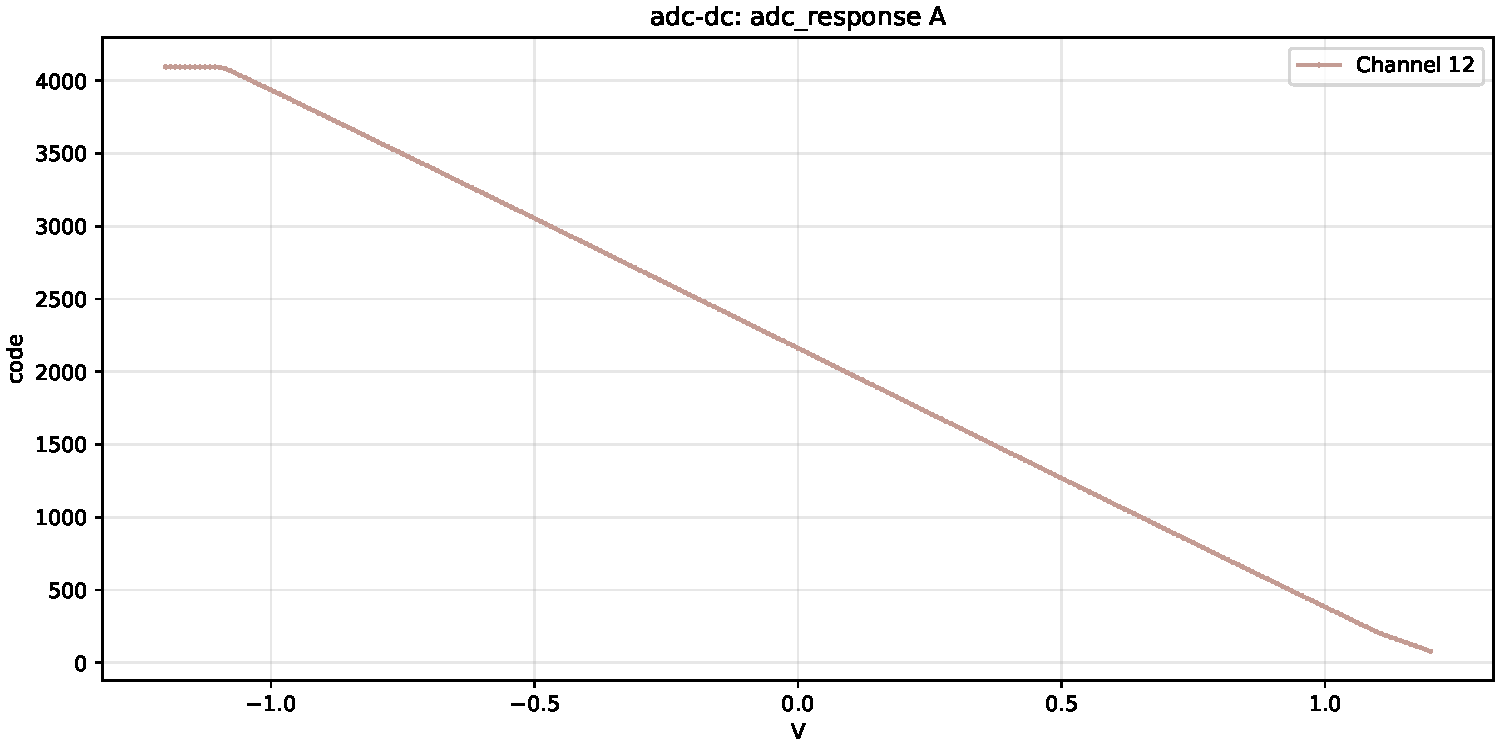
\includegraphics[width=\textwidth]{figures/figure-000.pdf}\end{center}
\begin{center}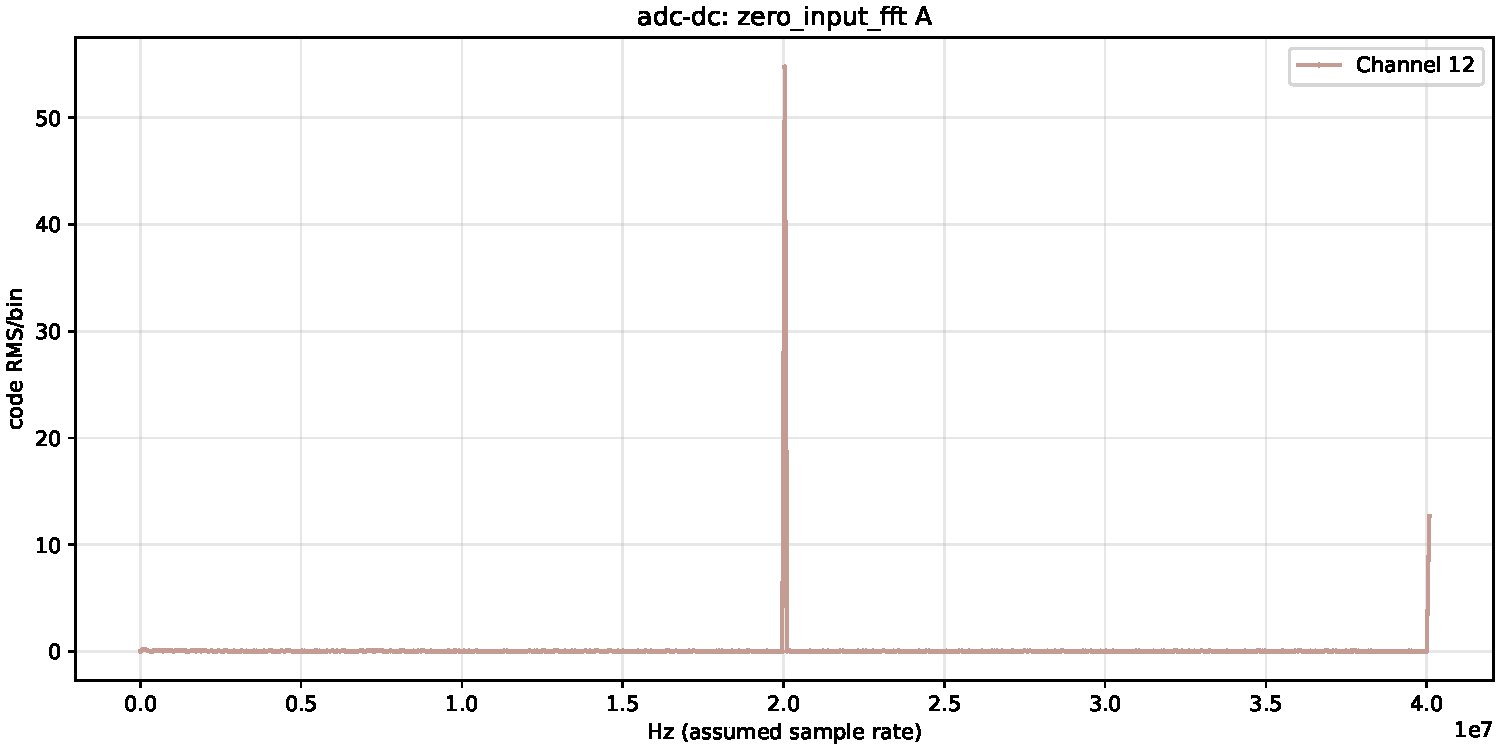
\includegraphics[width=\textwidth]{figures/figure-001.pdf}\end{center}
\begin{center}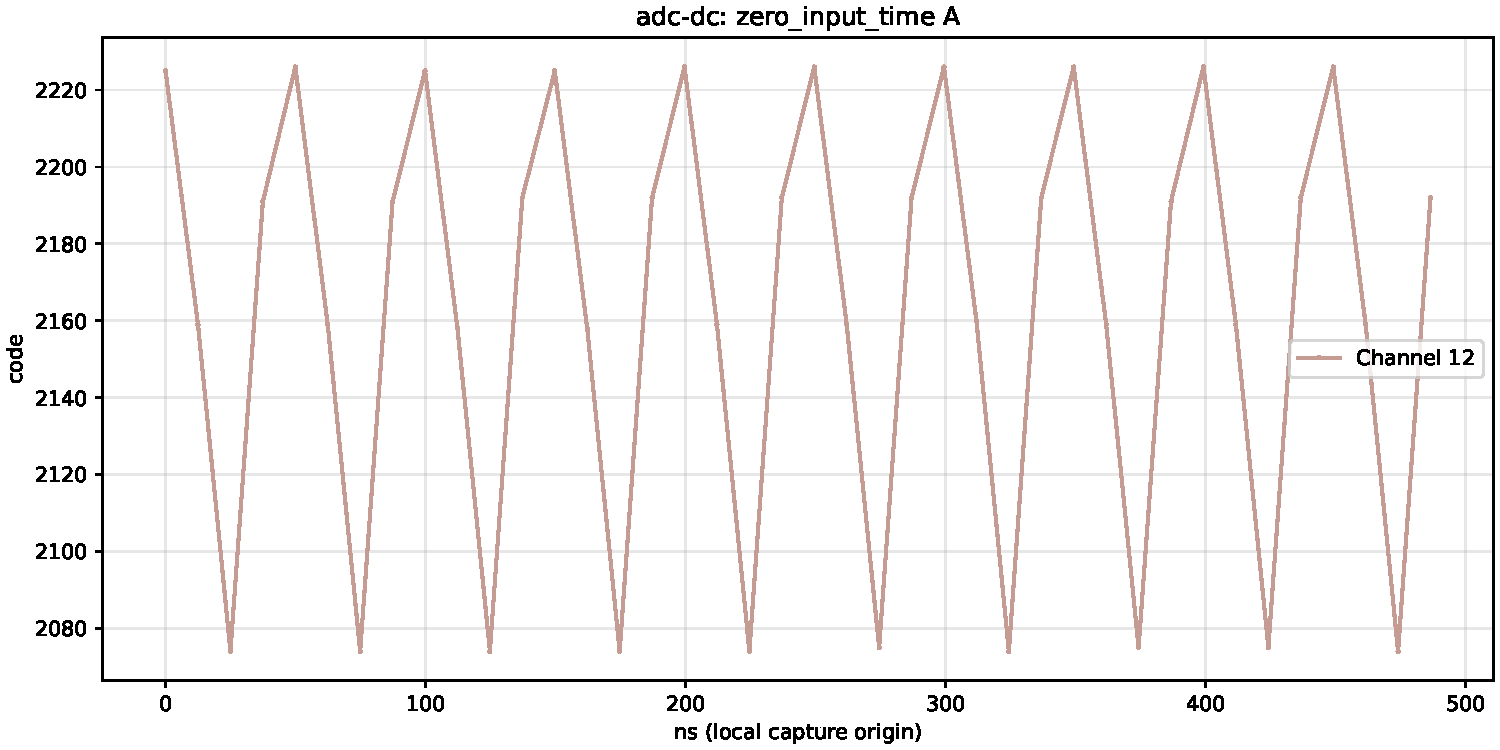
\includegraphics[width=\textwidth]{figures/figure-002.pdf}\end{center}
\begin{center}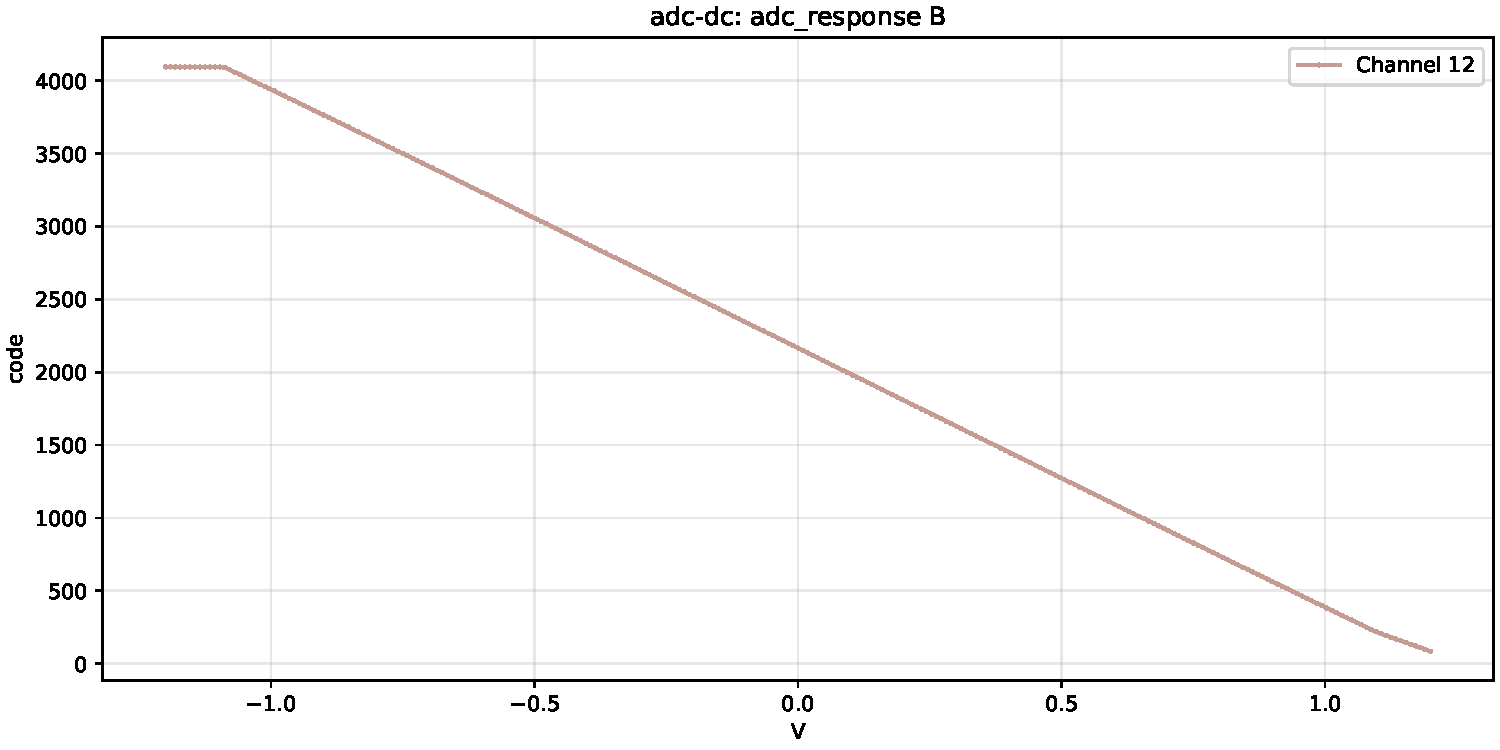
\includegraphics[width=\textwidth]{figures/figure-003.pdf}\end{center}
\begin{center}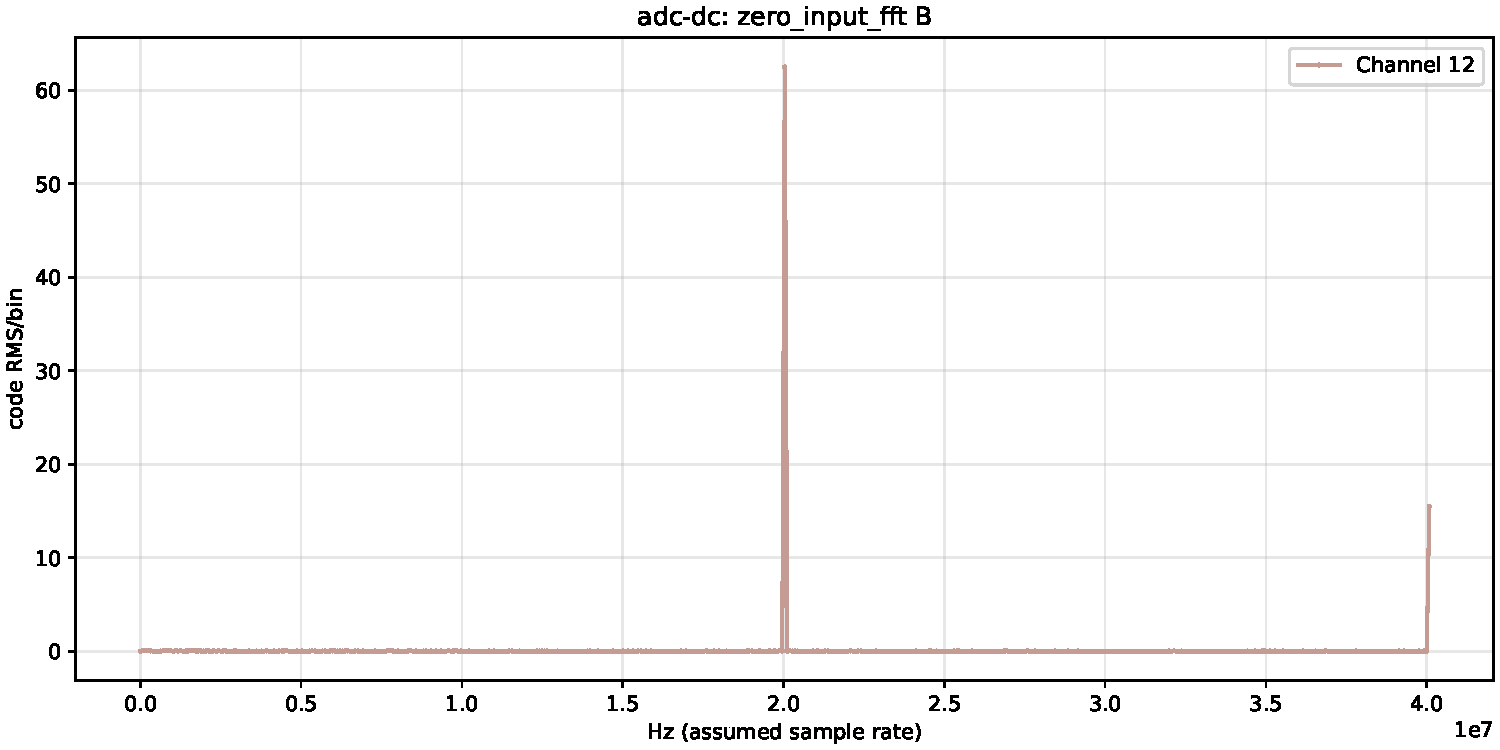
\includegraphics[width=\textwidth]{figures/figure-004.pdf}\end{center}
\begin{center}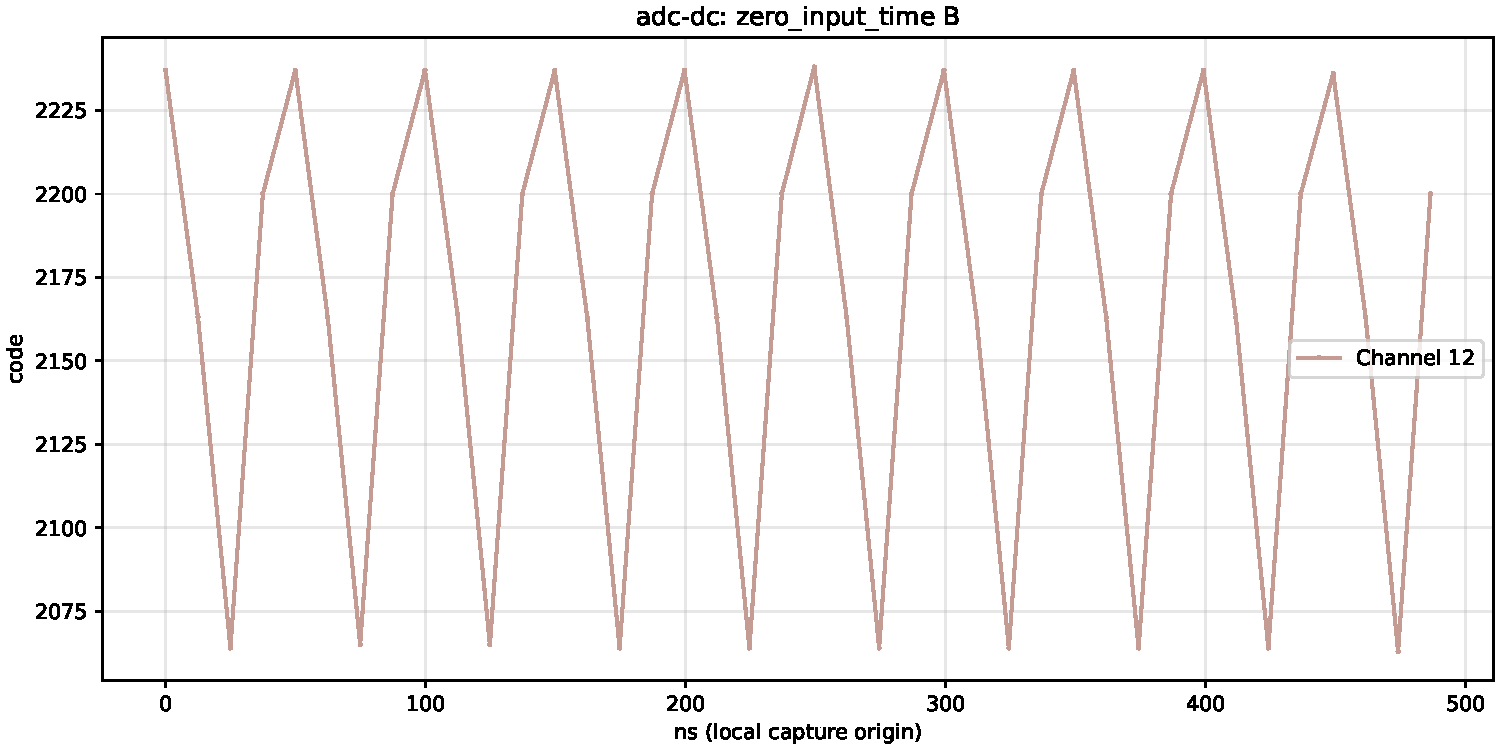
\includegraphics[width=\textwidth]{figures/figure-005.pdf}\end{center}
\begin{center}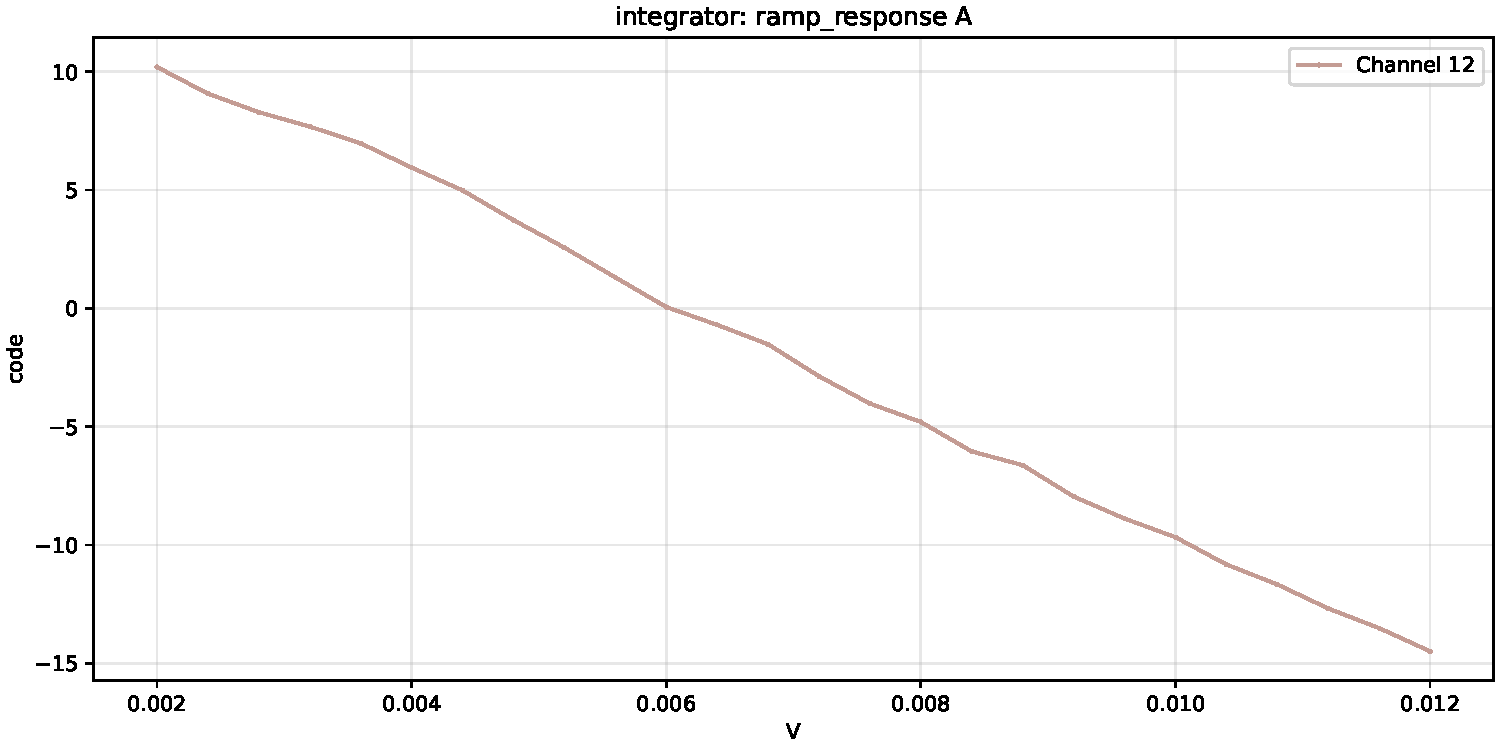
\includegraphics[width=\textwidth]{figures/figure-006.pdf}\end{center}
\begin{center}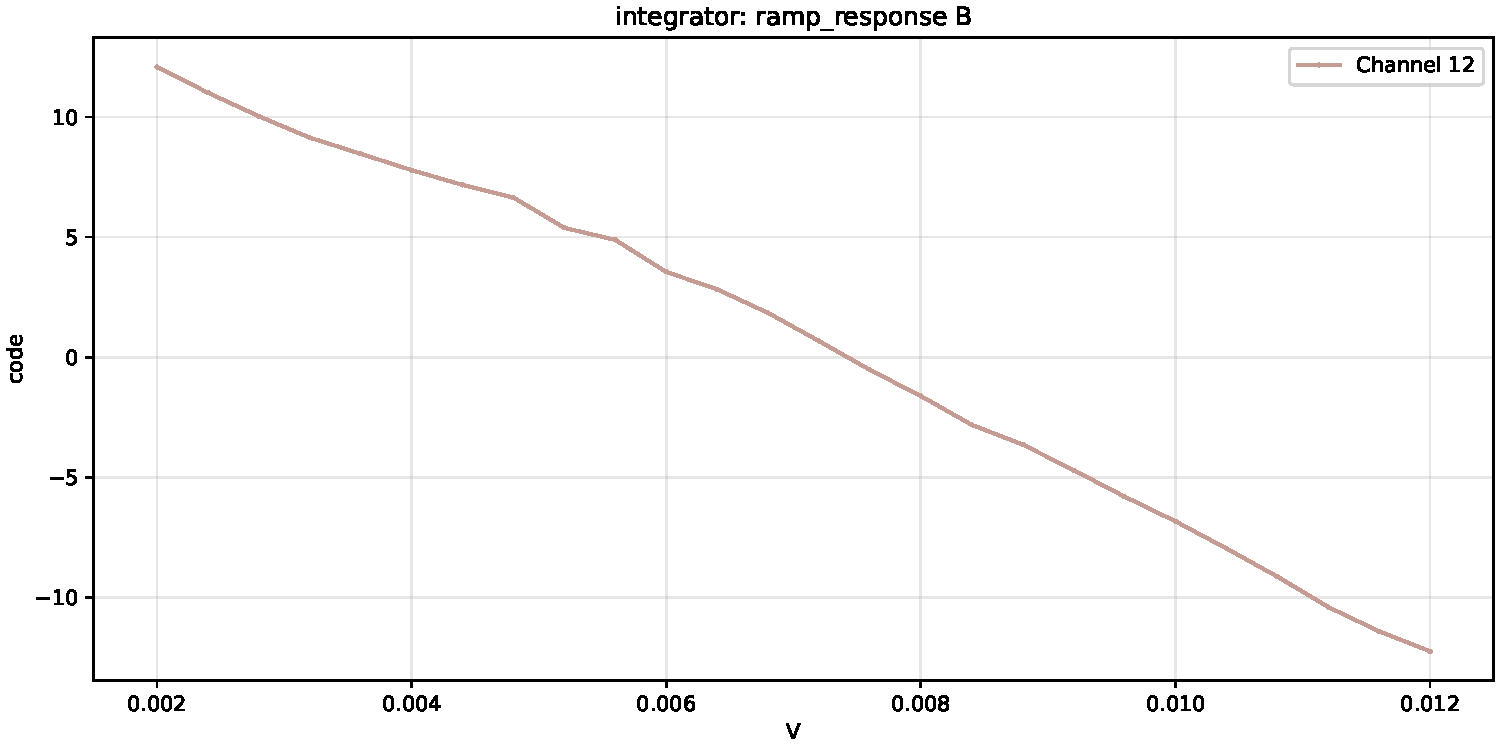
\includegraphics[width=\textwidth]{figures/figure-007.pdf}\end{center}
\begin{center}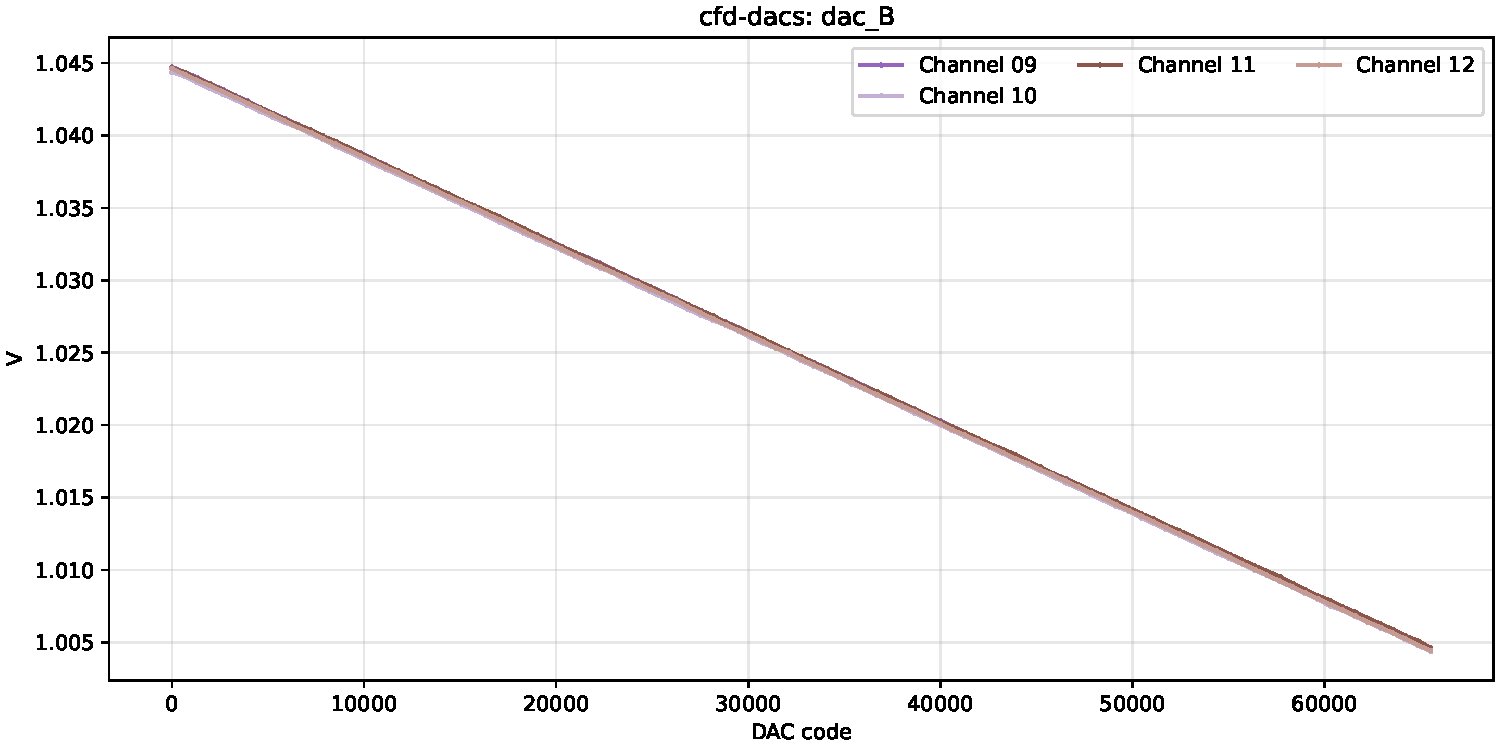
\includegraphics[width=\textwidth]{figures/figure-008.pdf}\end{center}
\begin{center}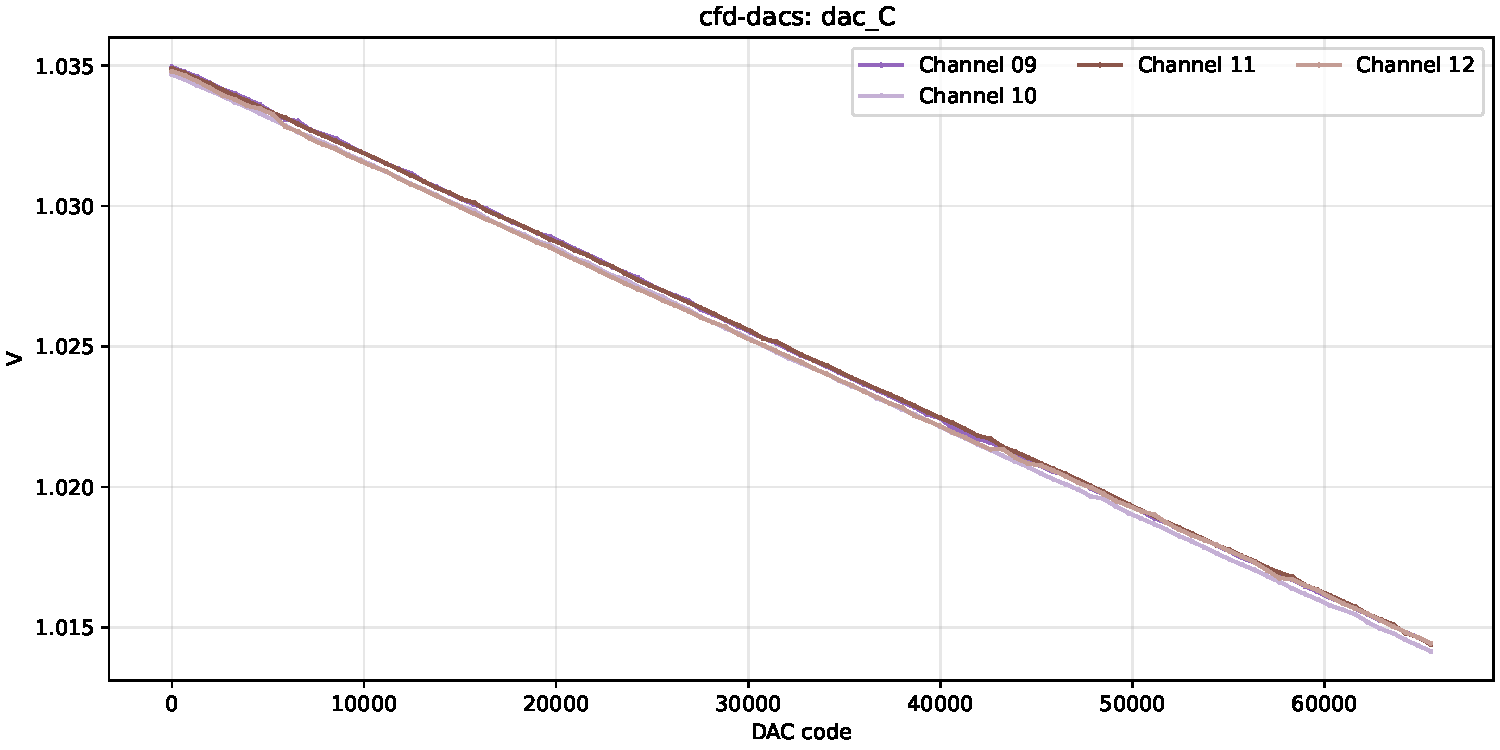
\includegraphics[width=\textwidth]{figures/figure-009.pdf}\end{center}
\begin{center}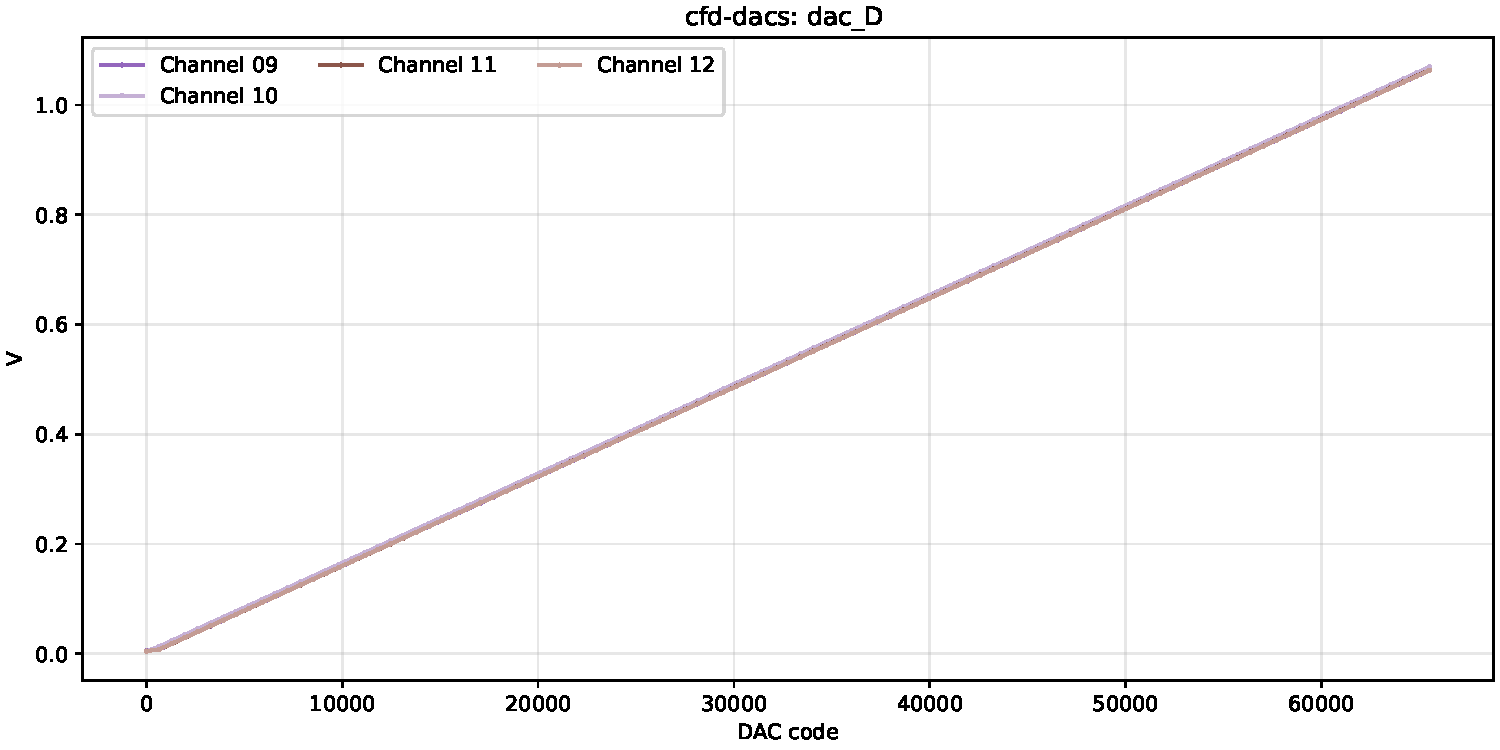
\includegraphics[width=\textwidth]{figures/figure-010.pdf}\end{center}
\begin{center}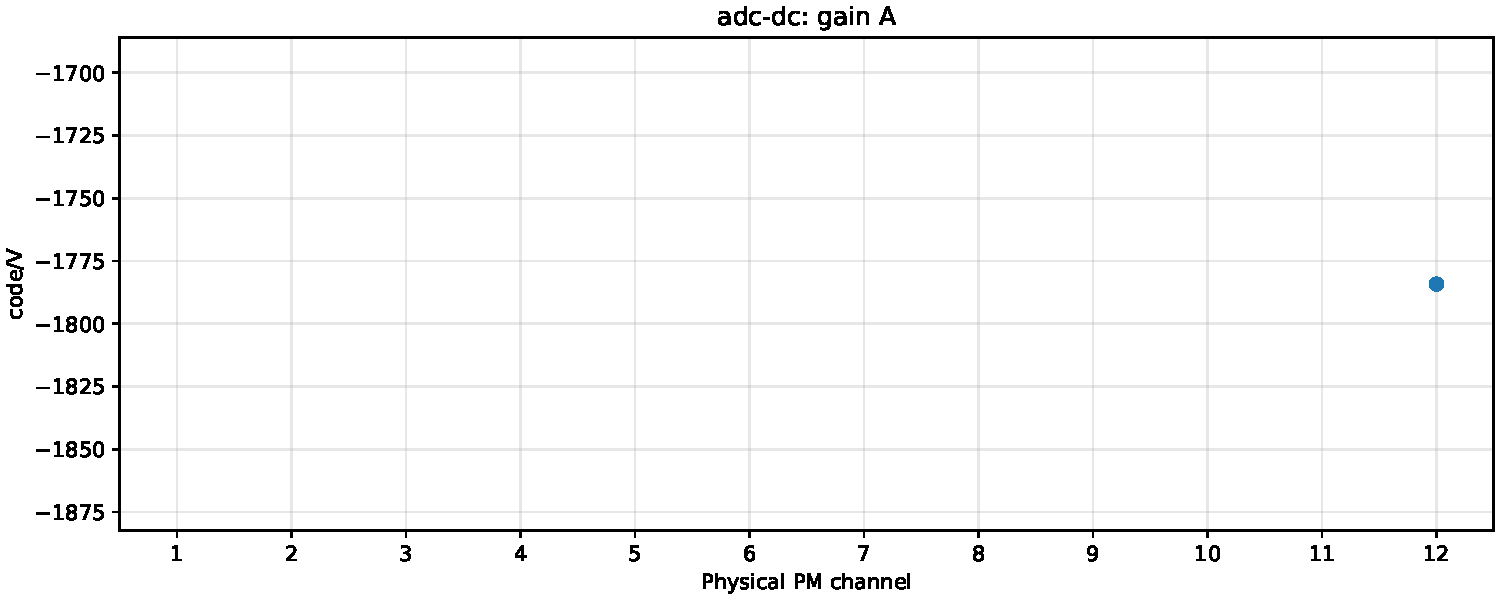
\includegraphics[width=\textwidth]{figures/figure-011.pdf}\end{center}
\begin{center}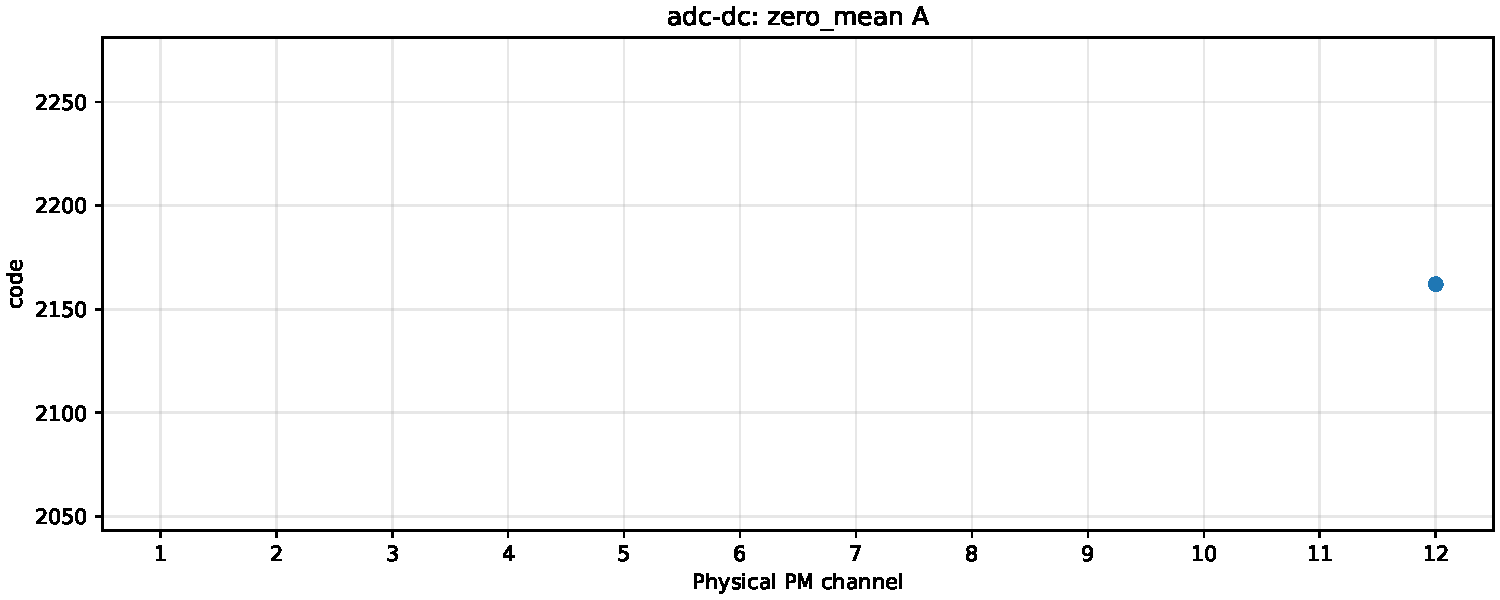
\includegraphics[width=\textwidth]{figures/figure-012.pdf}\end{center}
\begin{center}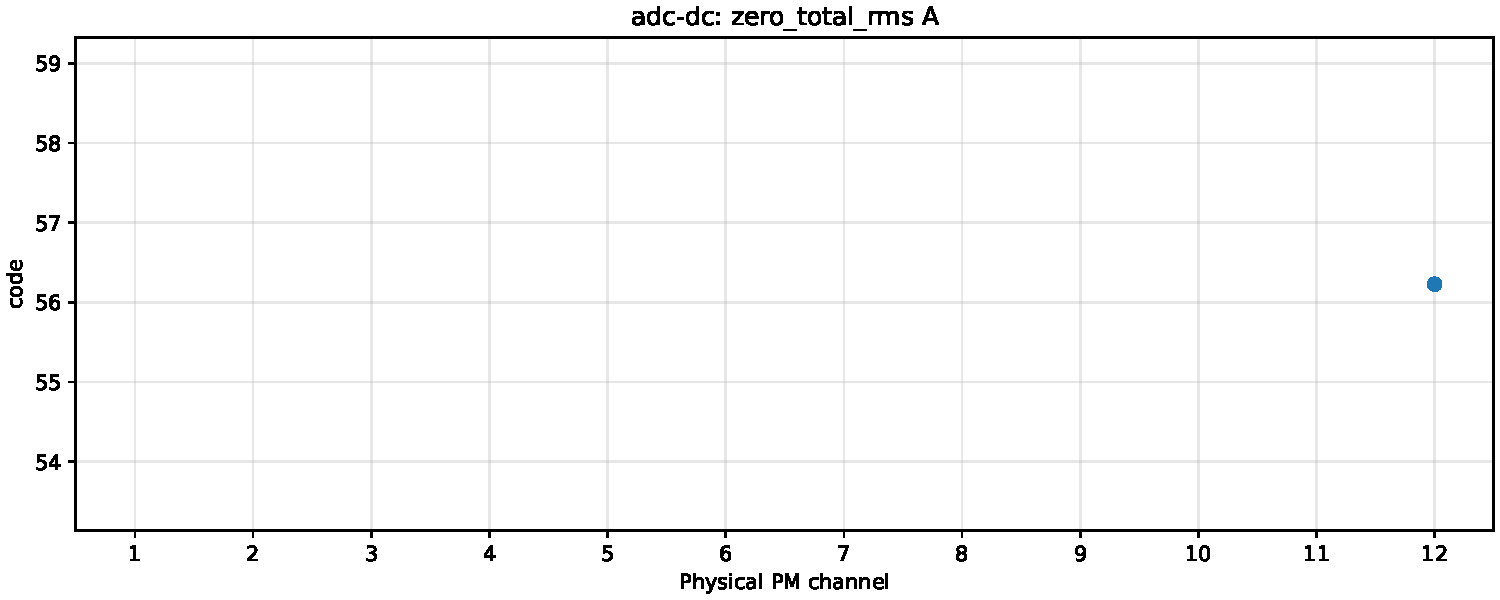
\includegraphics[width=\textwidth]{figures/figure-013.pdf}\end{center}
\begin{center}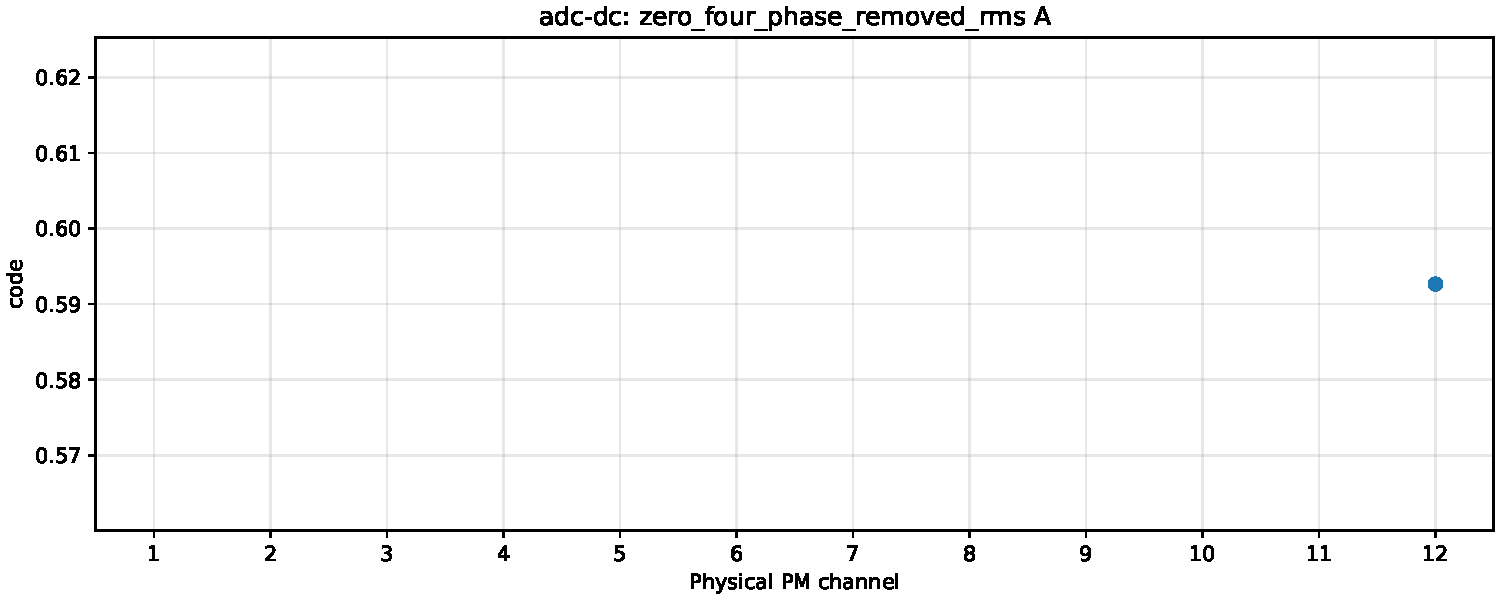
\includegraphics[width=\textwidth]{figures/figure-014.pdf}\end{center}
\begin{center}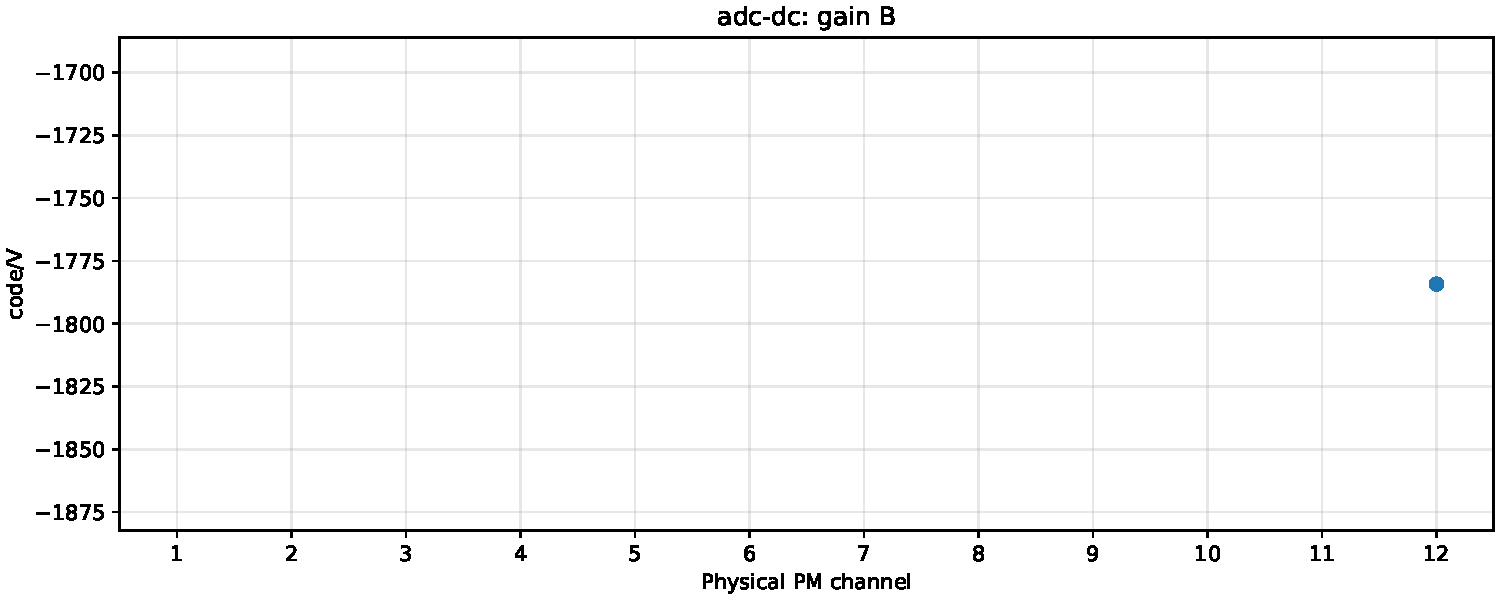
\includegraphics[width=\textwidth]{figures/figure-015.pdf}\end{center}
\begin{center}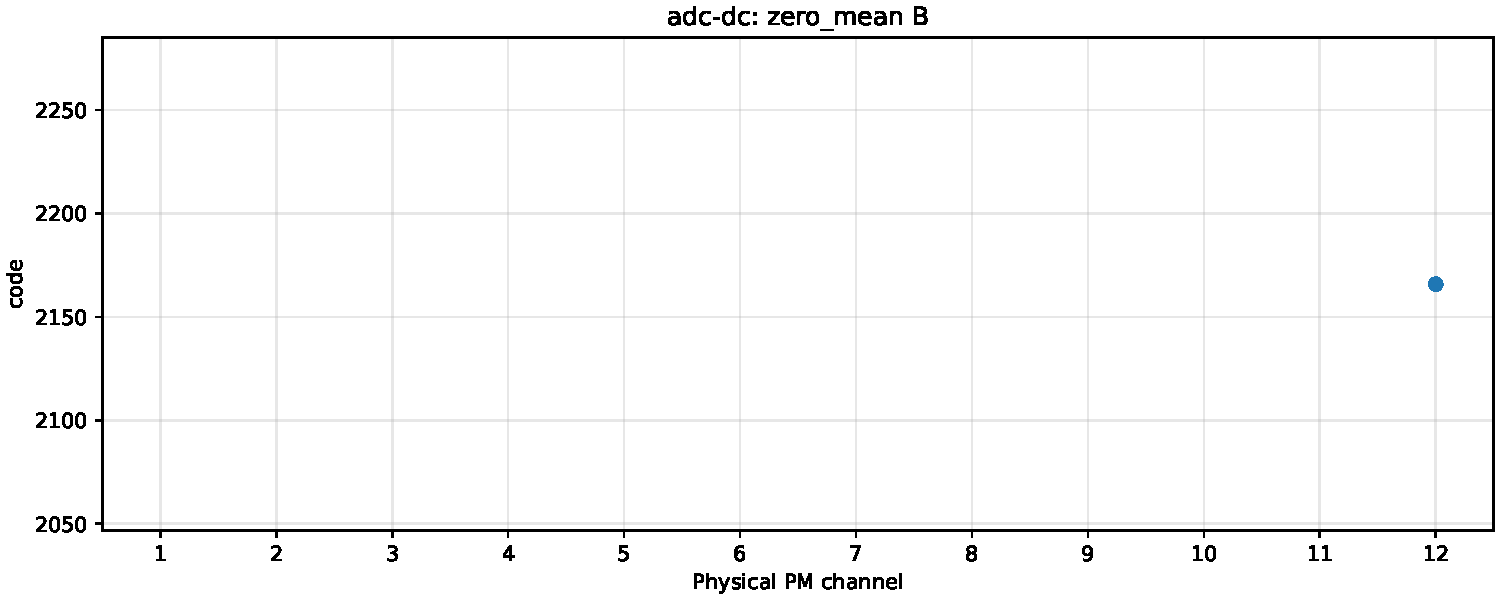
\includegraphics[width=\textwidth]{figures/figure-016.pdf}\end{center}
\begin{center}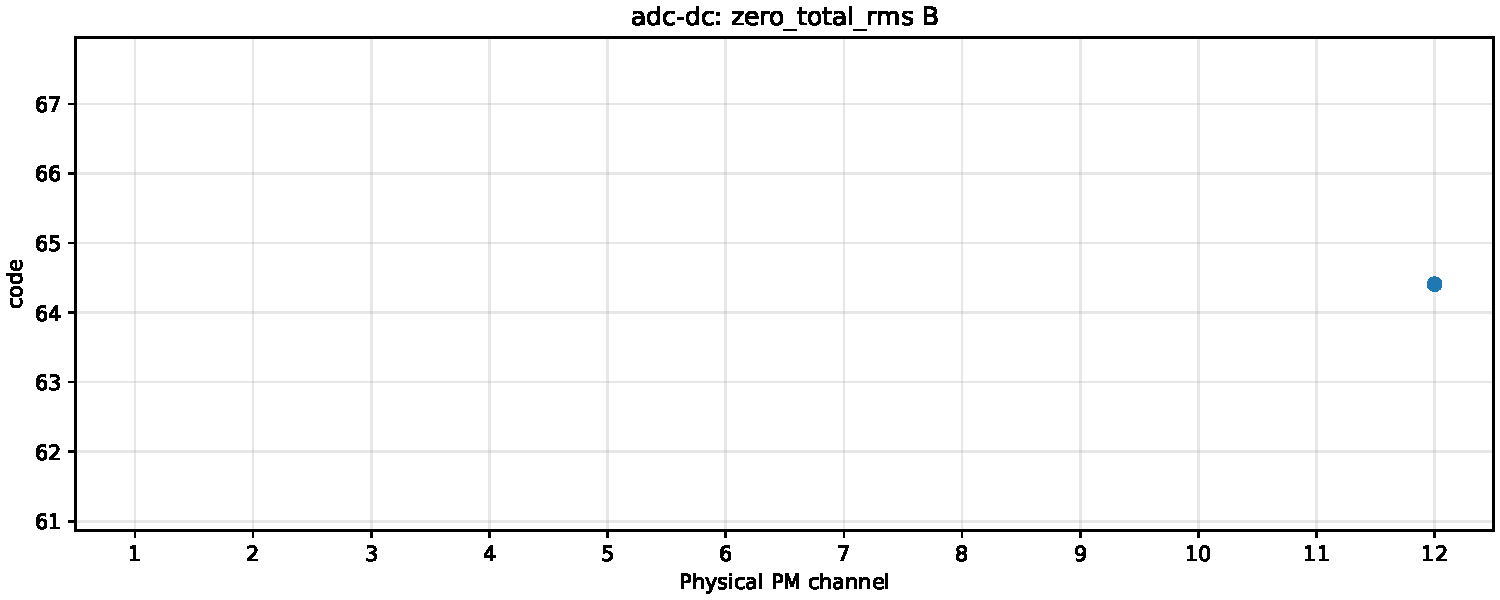
\includegraphics[width=\textwidth]{figures/figure-017.pdf}\end{center}
\begin{center}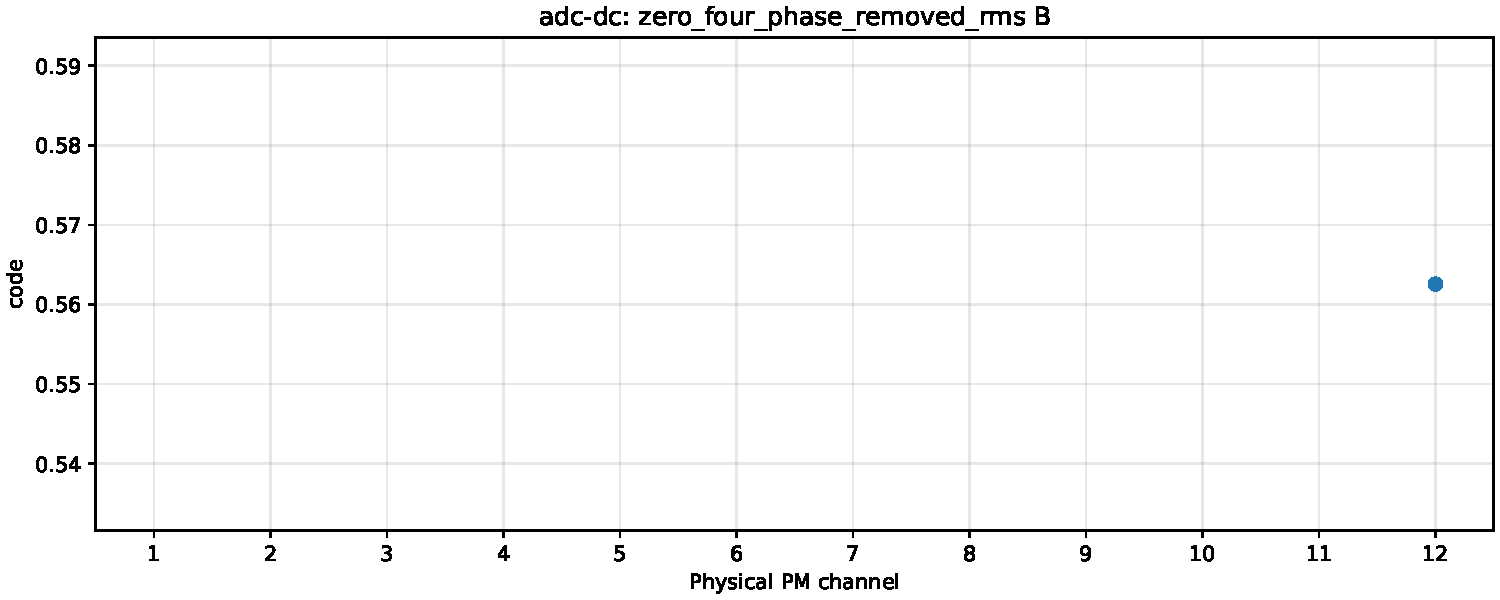
\includegraphics[width=\textwidth]{figures/figure-018.pdf}\end{center}
\begin{center}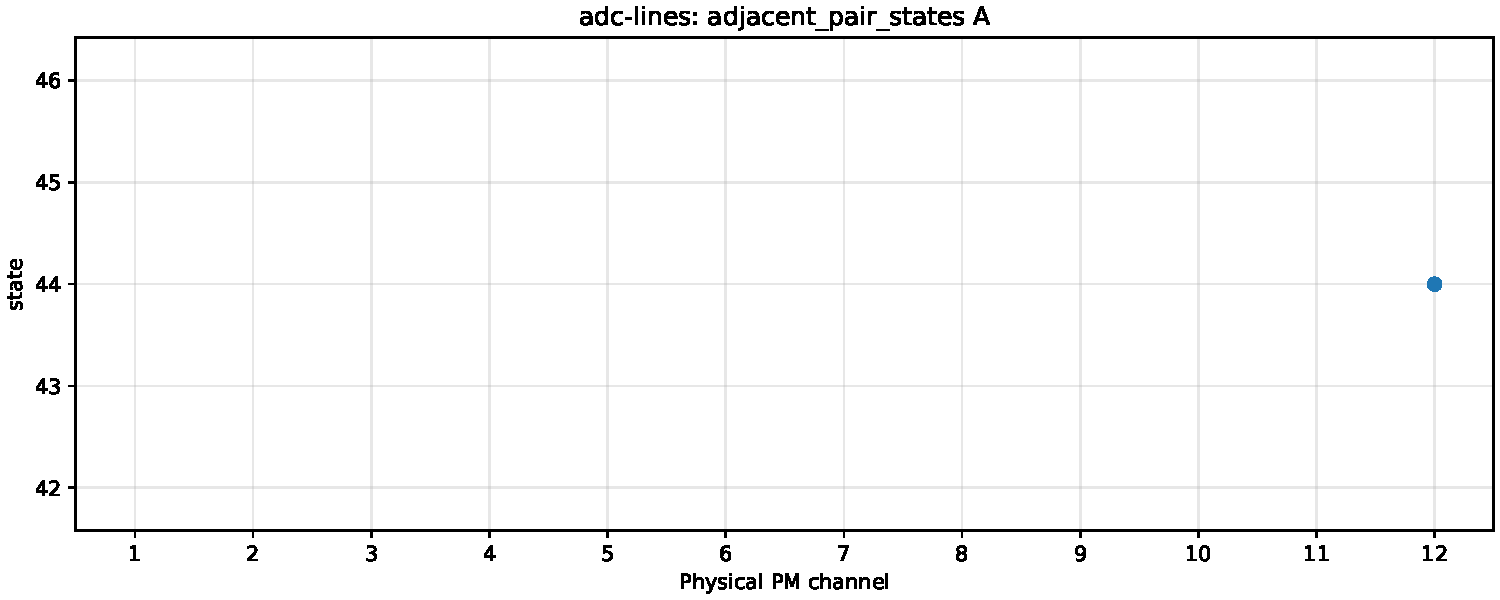
\includegraphics[width=\textwidth]{figures/figure-019.pdf}\end{center}
\begin{center}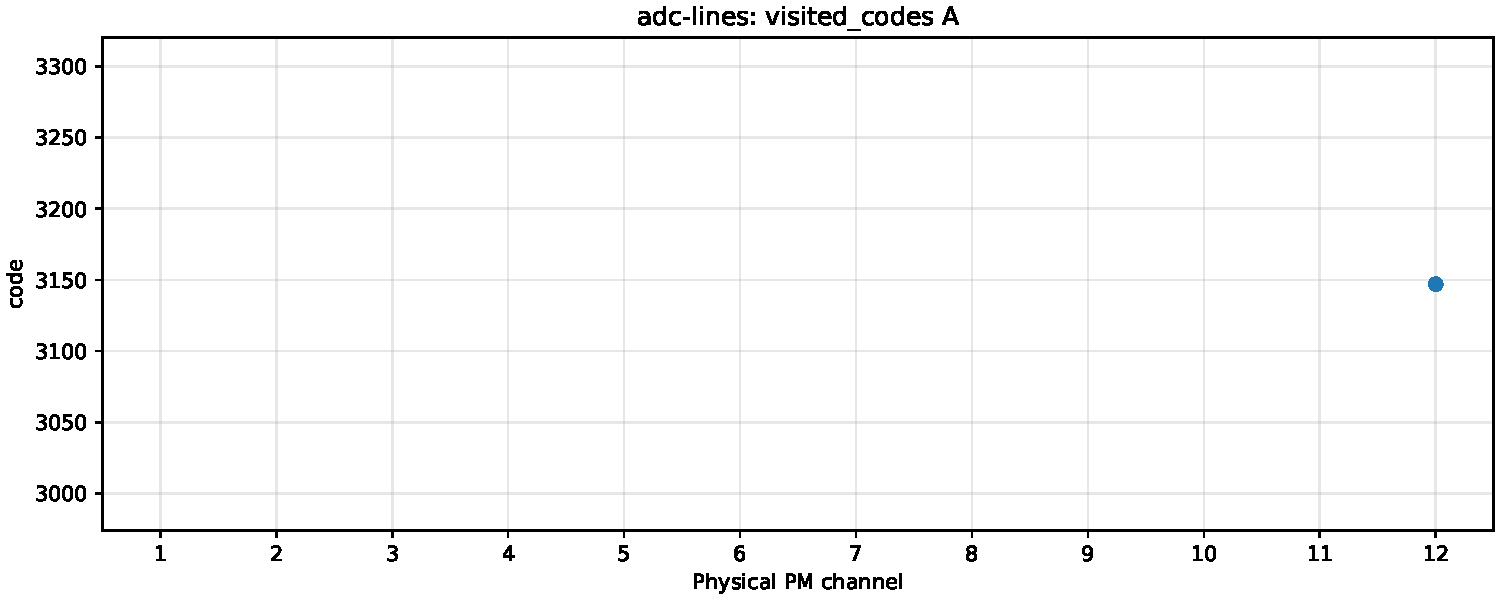
\includegraphics[width=\textwidth]{figures/figure-020.pdf}\end{center}
\begin{center}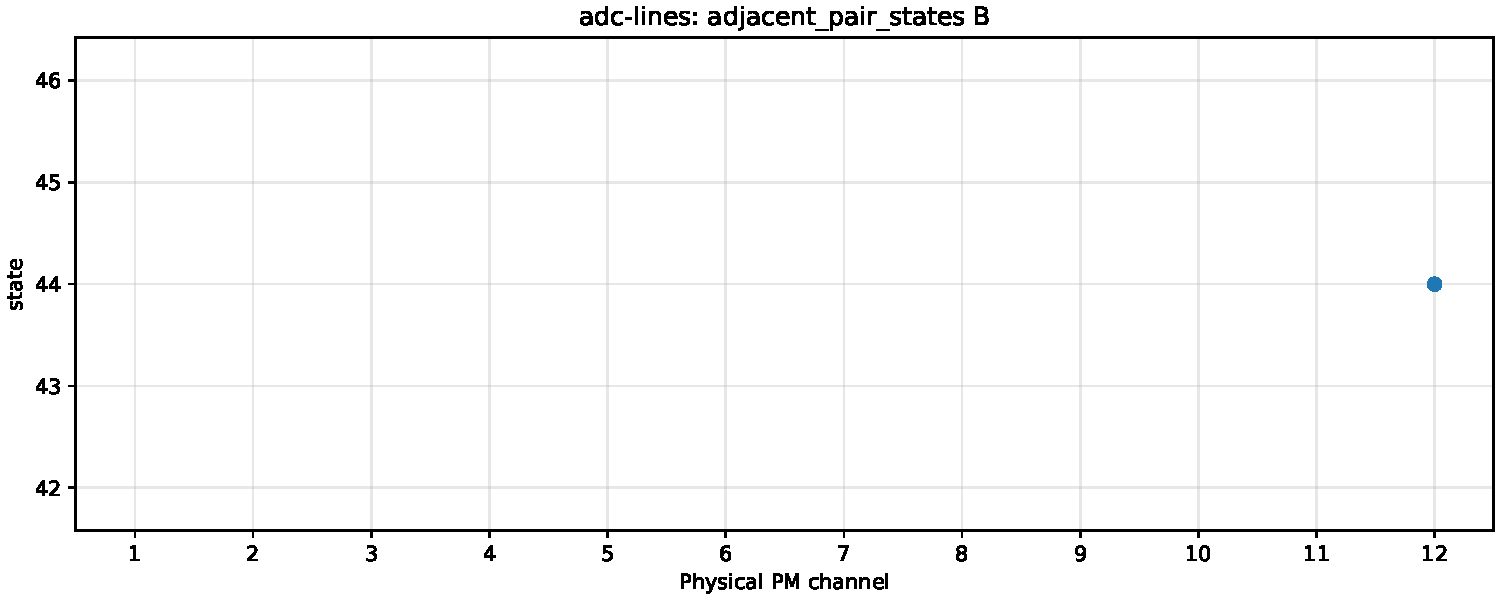
\includegraphics[width=\textwidth]{figures/figure-021.pdf}\end{center}
\begin{center}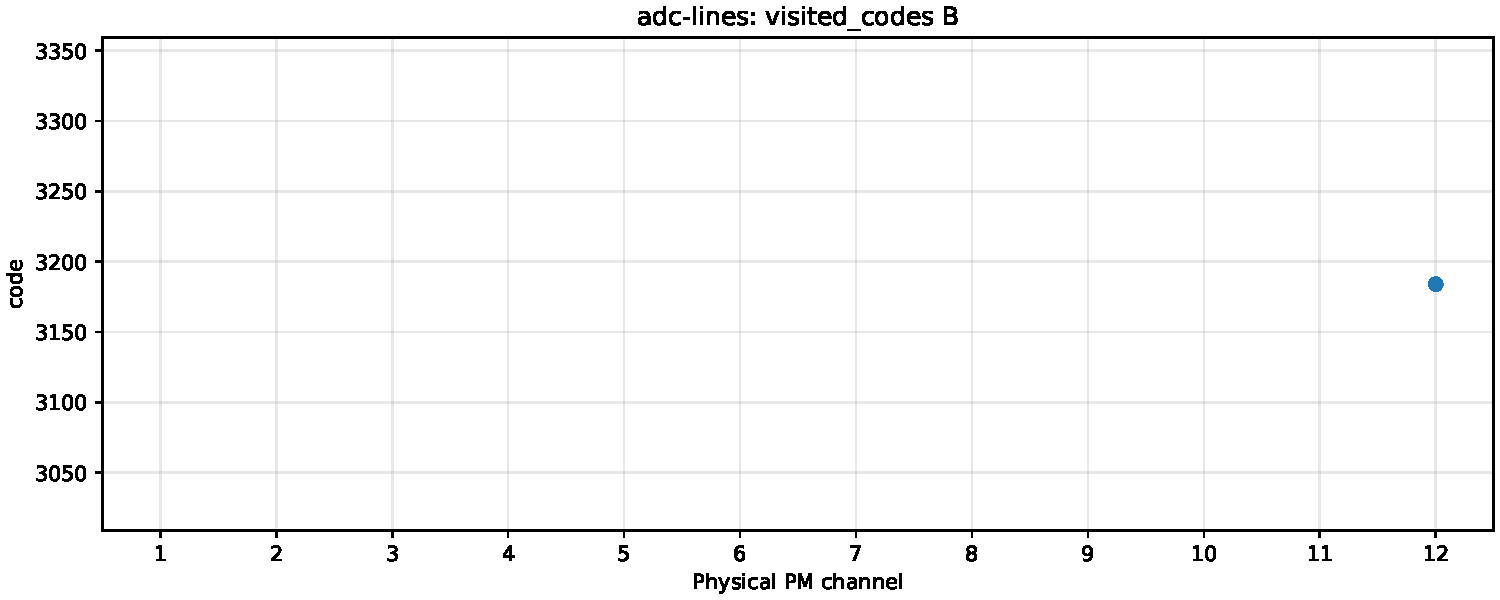
\includegraphics[width=\textwidth]{figures/figure-022.pdf}\end{center}
\begin{center}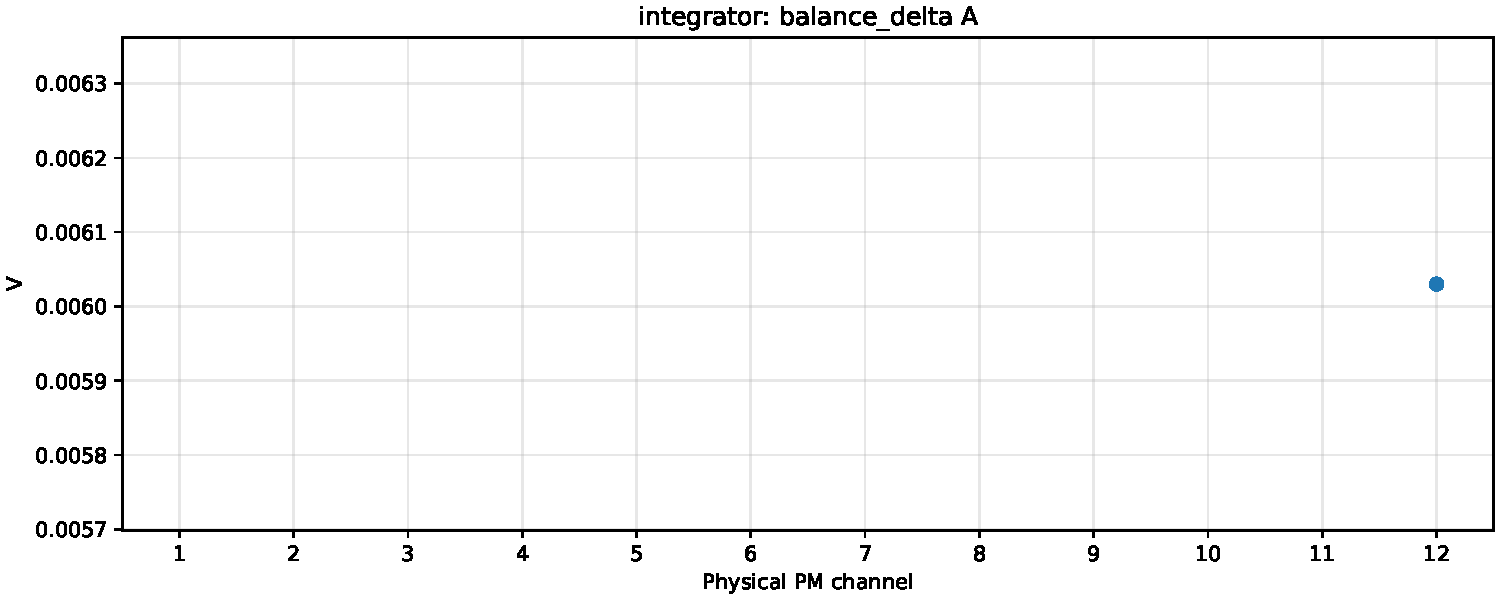
\includegraphics[width=\textwidth]{figures/figure-023.pdf}\end{center}
\begin{center}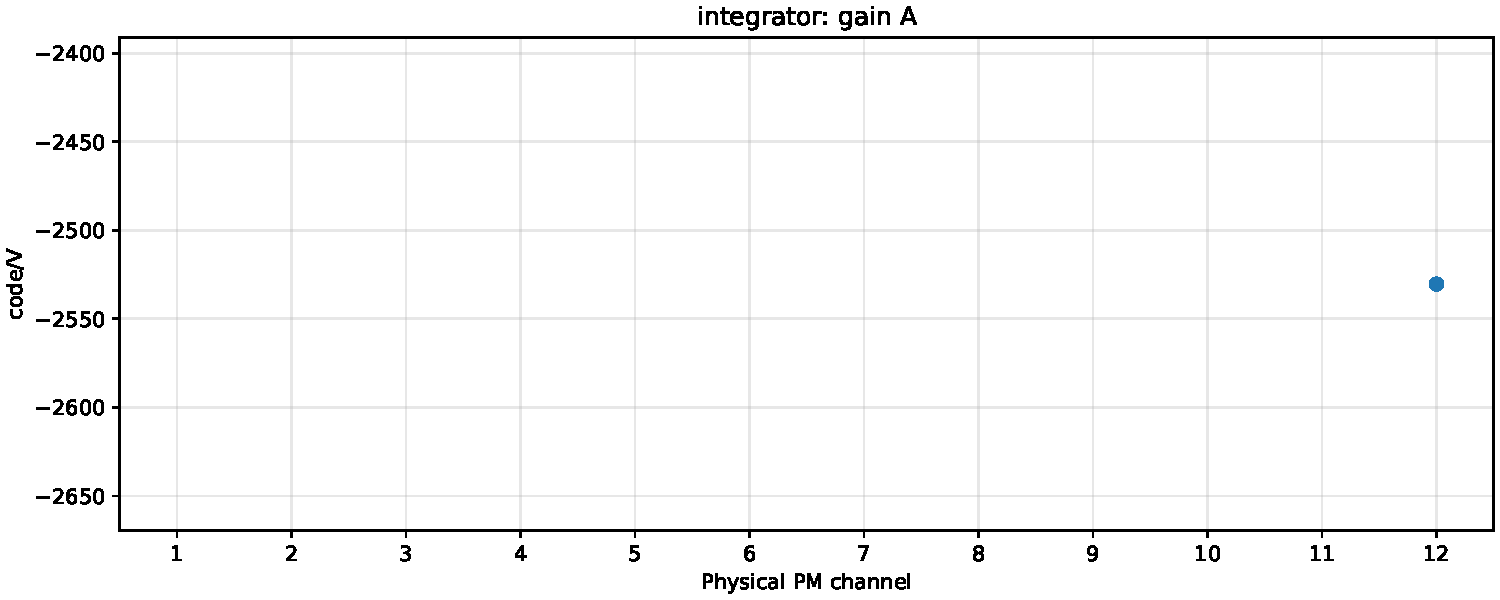
\includegraphics[width=\textwidth]{figures/figure-024.pdf}\end{center}
\begin{center}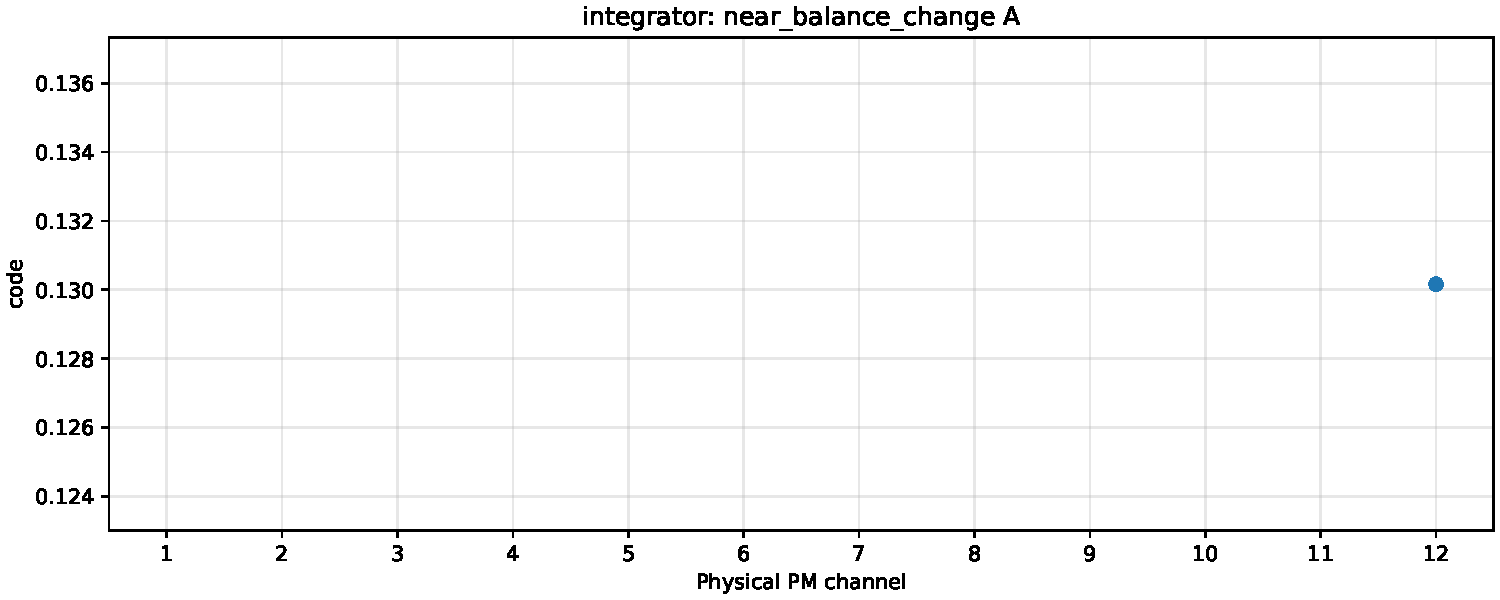
\includegraphics[width=\textwidth]{figures/figure-025.pdf}\end{center}
\begin{center}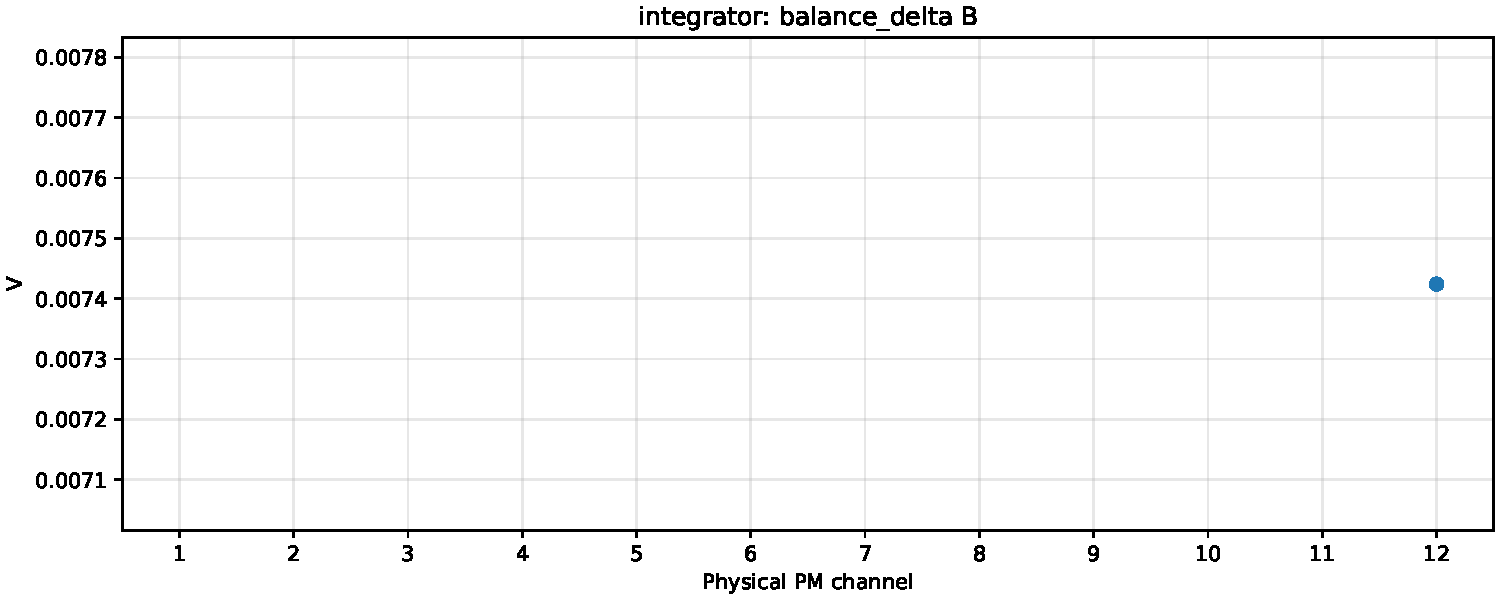
\includegraphics[width=\textwidth]{figures/figure-026.pdf}\end{center}
\begin{center}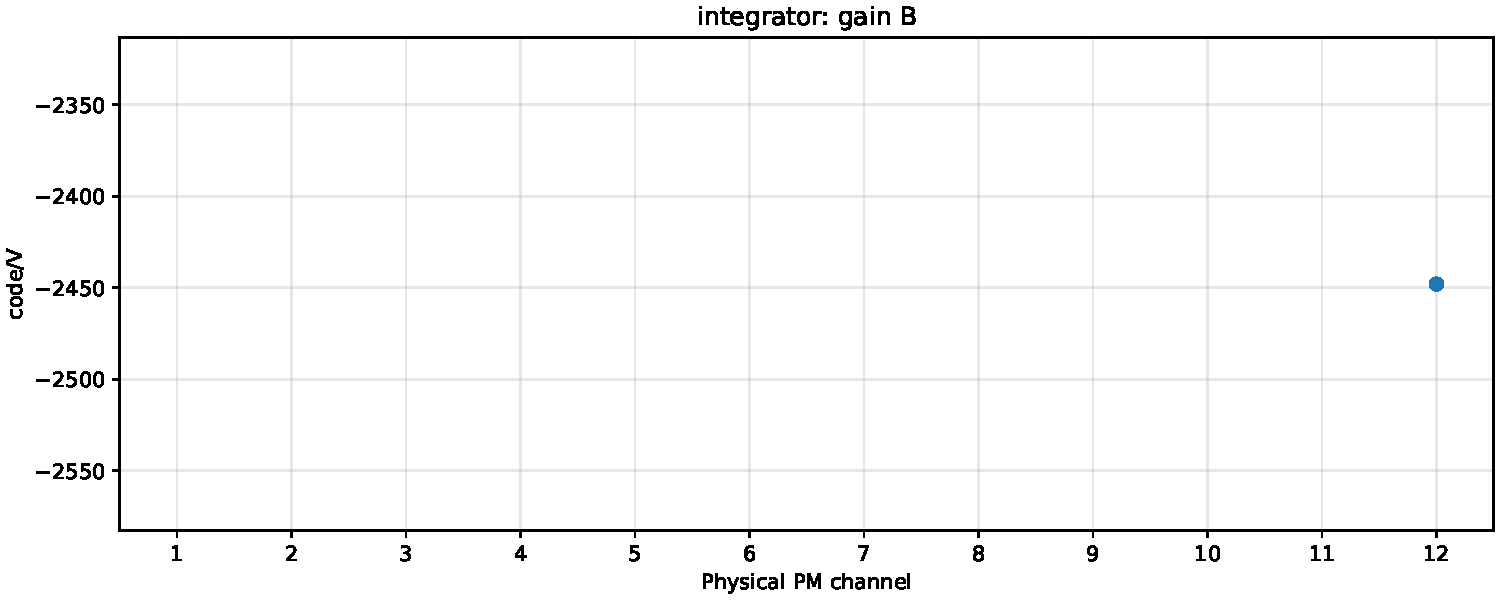
\includegraphics[width=\textwidth]{figures/figure-027.pdf}\end{center}
\begin{center}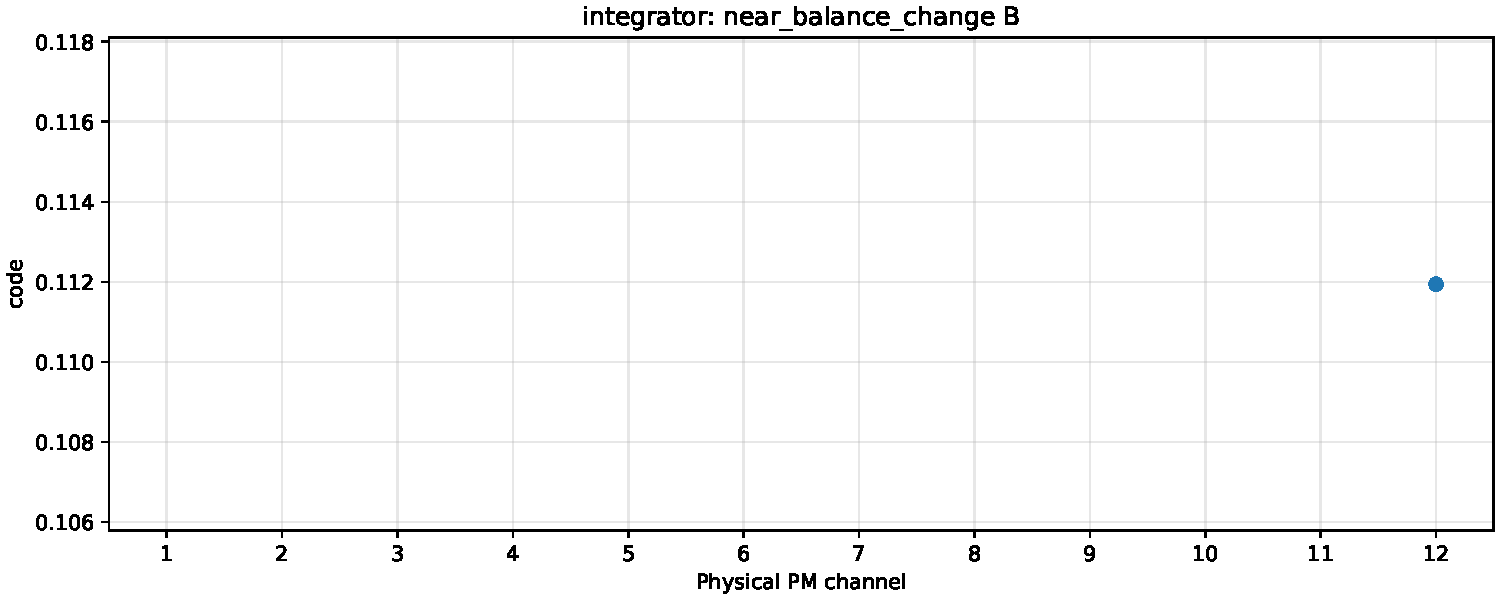
\includegraphics[width=\textwidth]{figures/figure-028.pdf}\end{center}
\begin{center}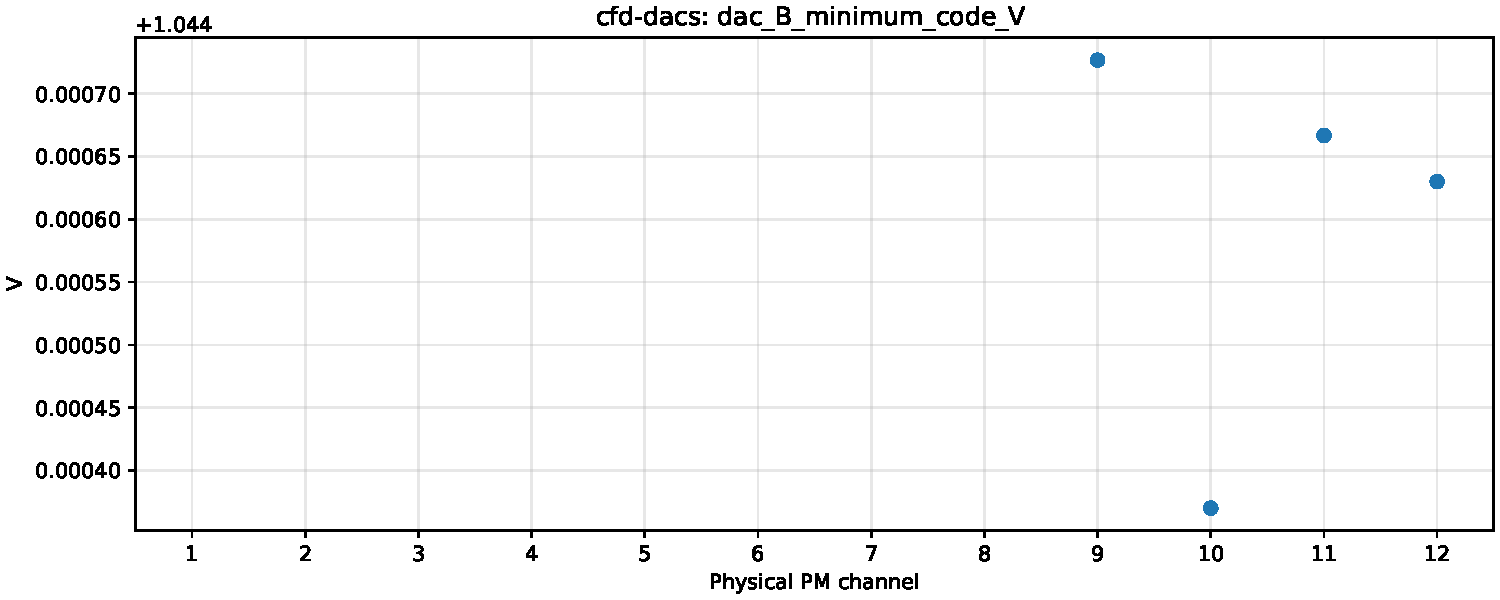
\includegraphics[width=\textwidth]{figures/figure-029.pdf}\end{center}
\begin{center}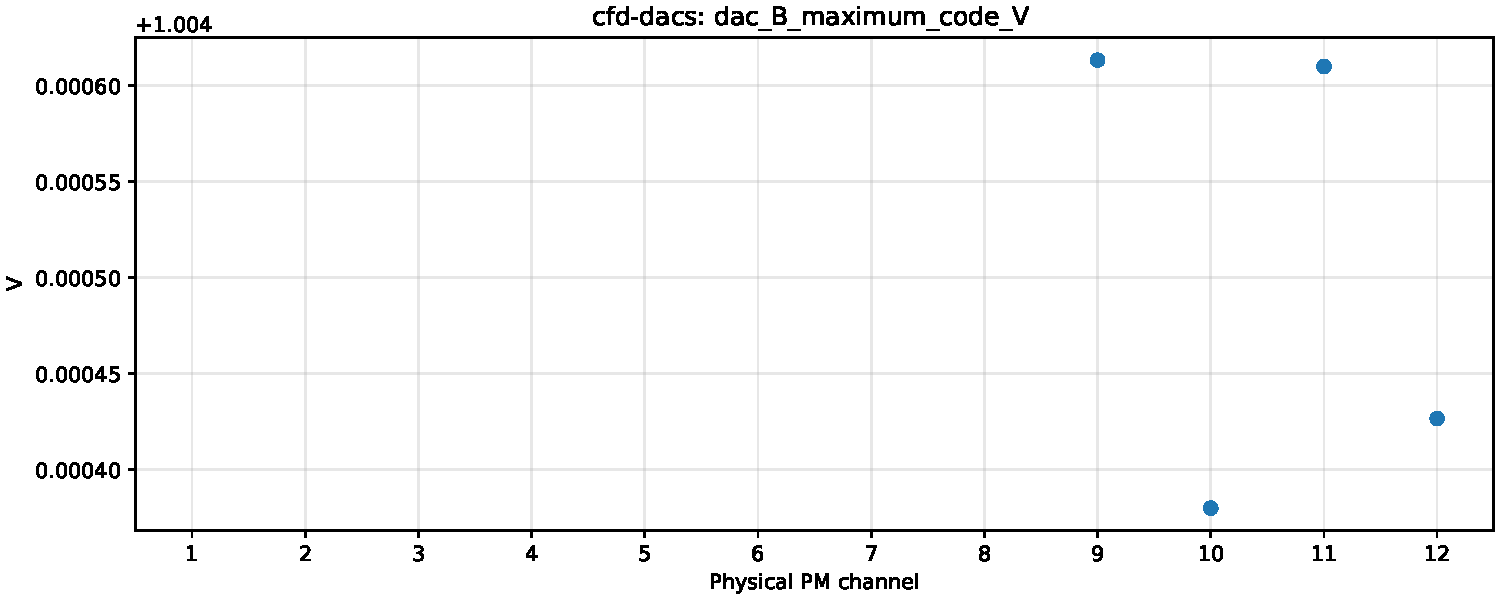
\includegraphics[width=\textwidth]{figures/figure-030.pdf}\end{center}
\begin{center}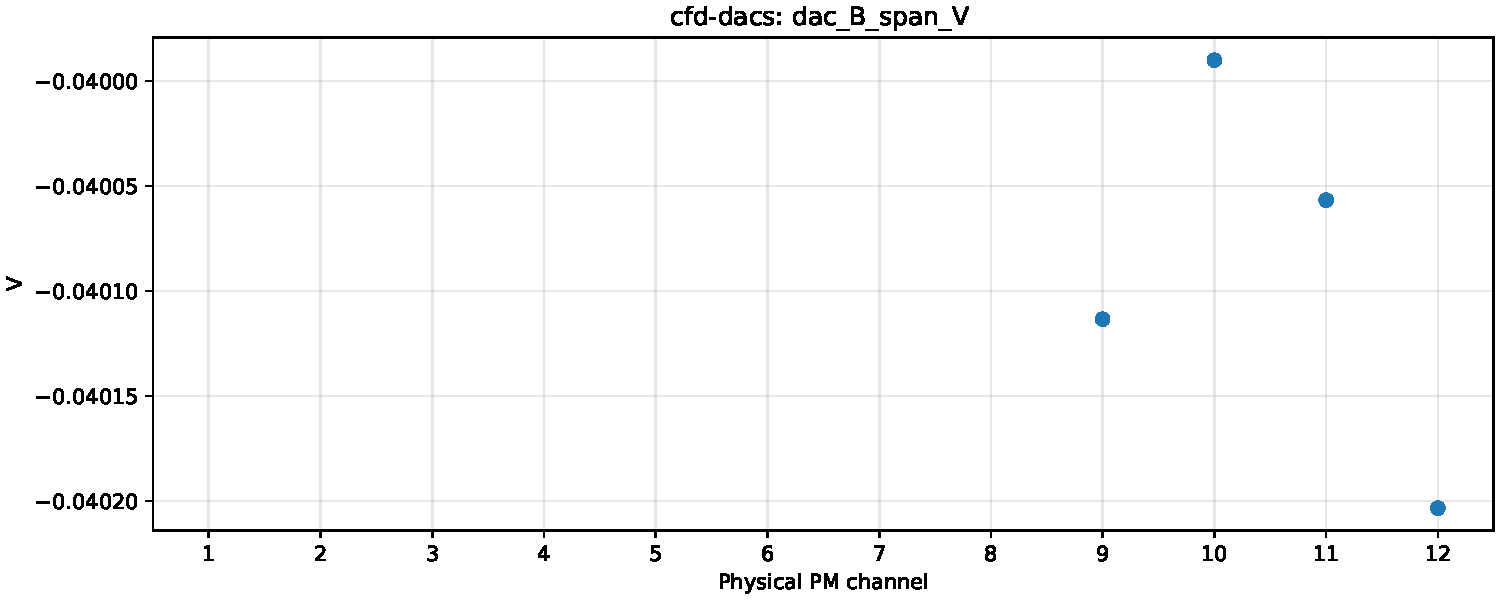
\includegraphics[width=\textwidth]{figures/figure-031.pdf}\end{center}
\begin{center}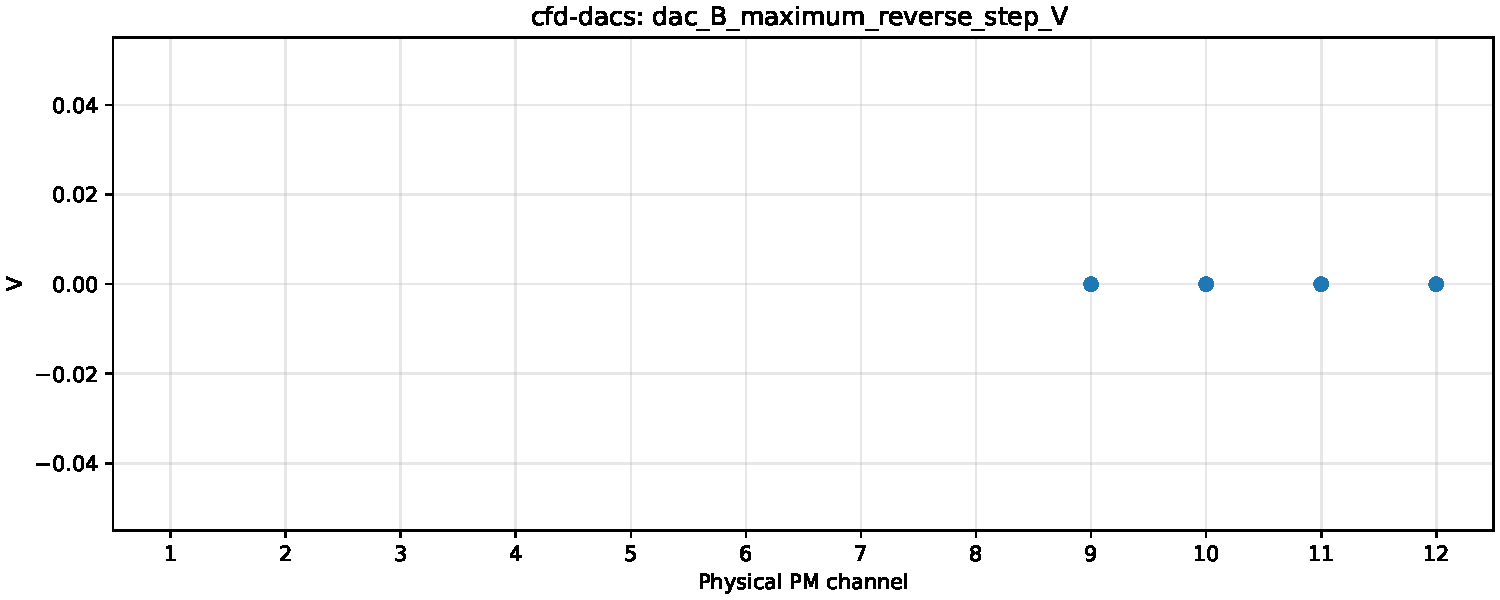
\includegraphics[width=\textwidth]{figures/figure-032.pdf}\end{center}
\begin{center}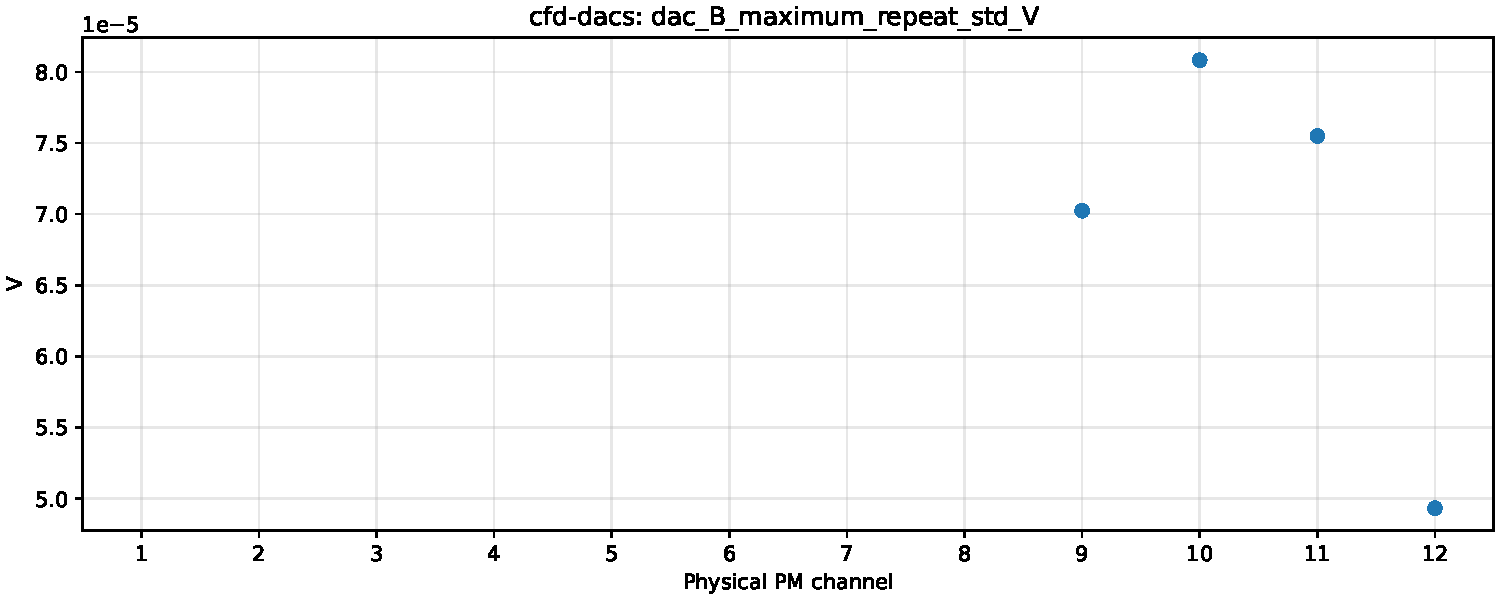
\includegraphics[width=\textwidth]{figures/figure-033.pdf}\end{center}
\begin{center}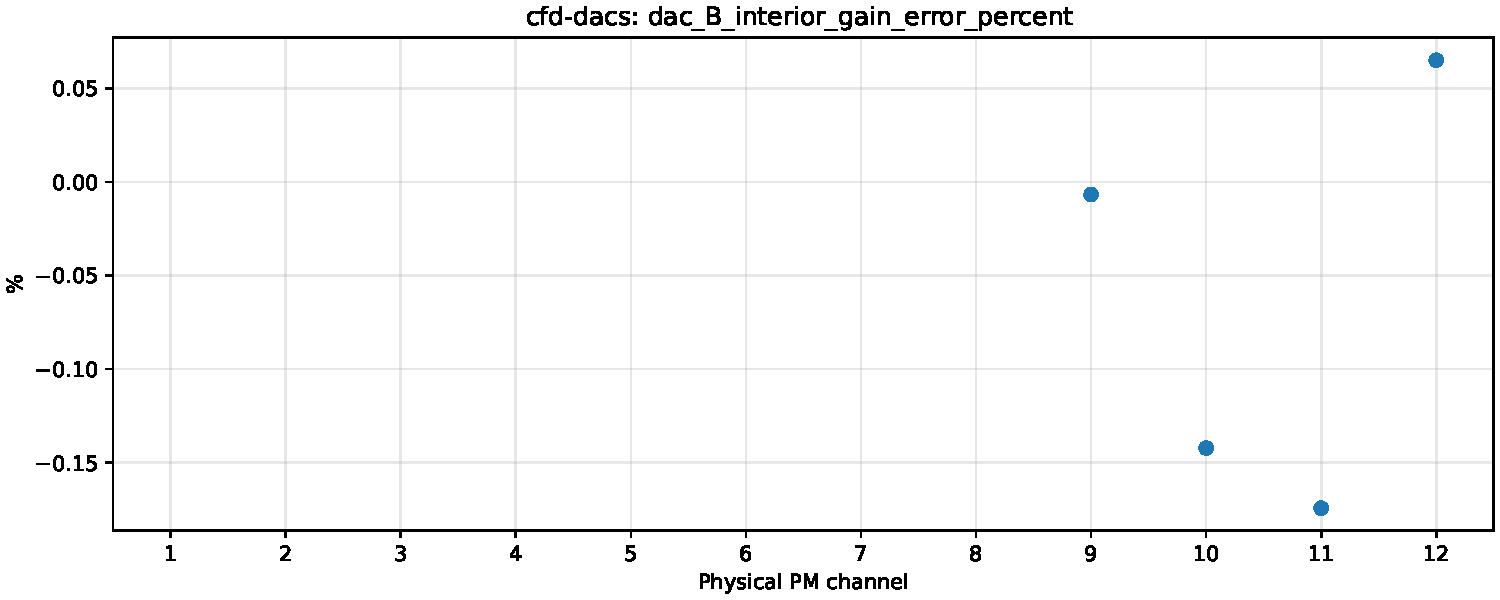
\includegraphics[width=\textwidth]{figures/figure-034.pdf}\end{center}
\begin{center}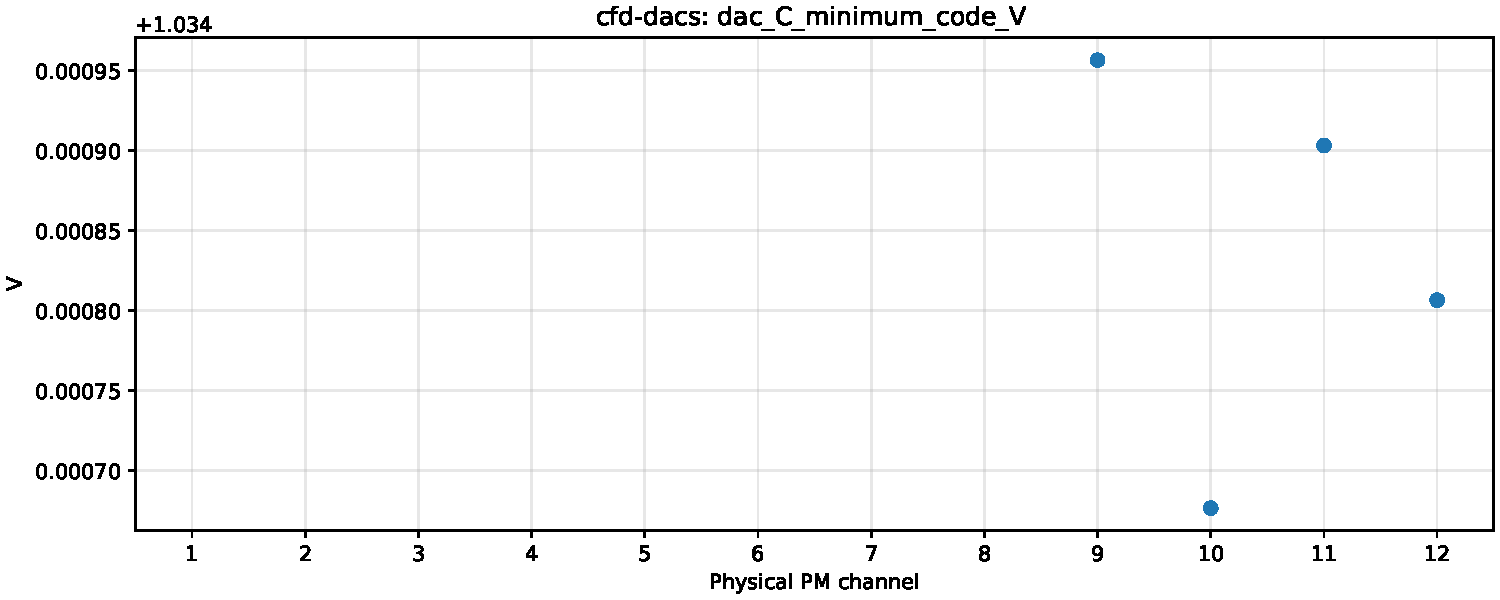
\includegraphics[width=\textwidth]{figures/figure-035.pdf}\end{center}
\begin{center}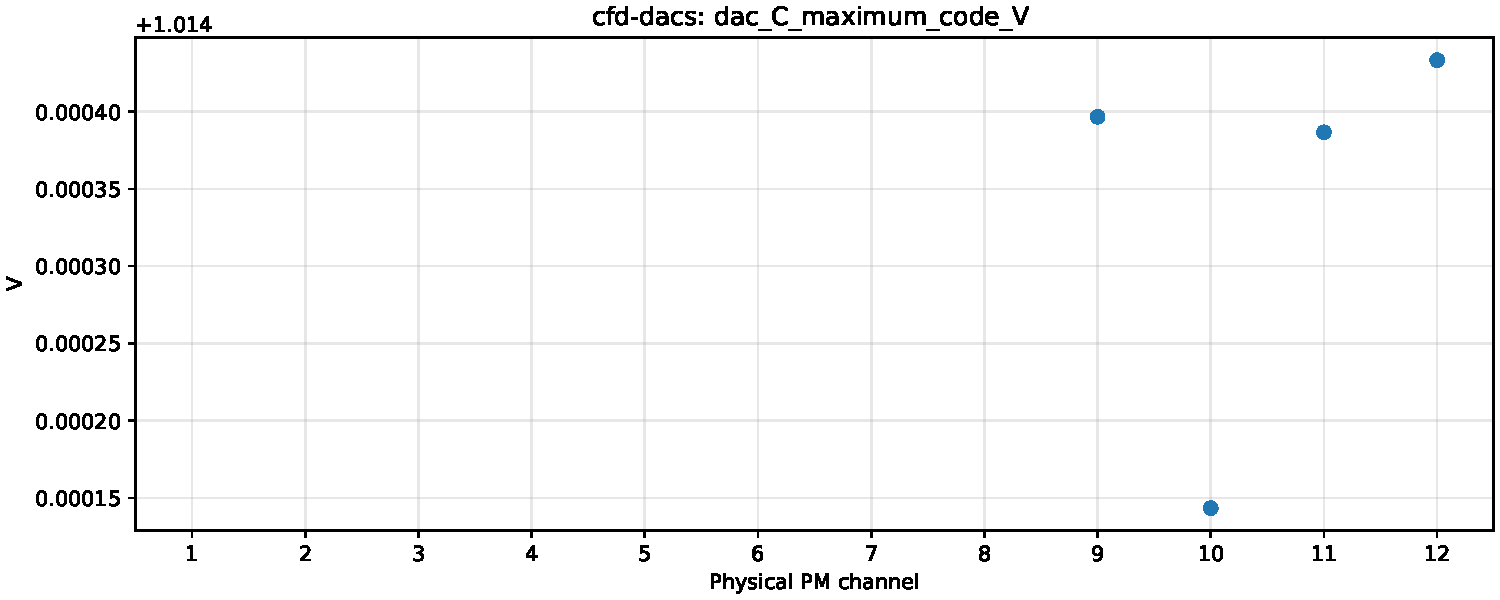
\includegraphics[width=\textwidth]{figures/figure-036.pdf}\end{center}
\begin{center}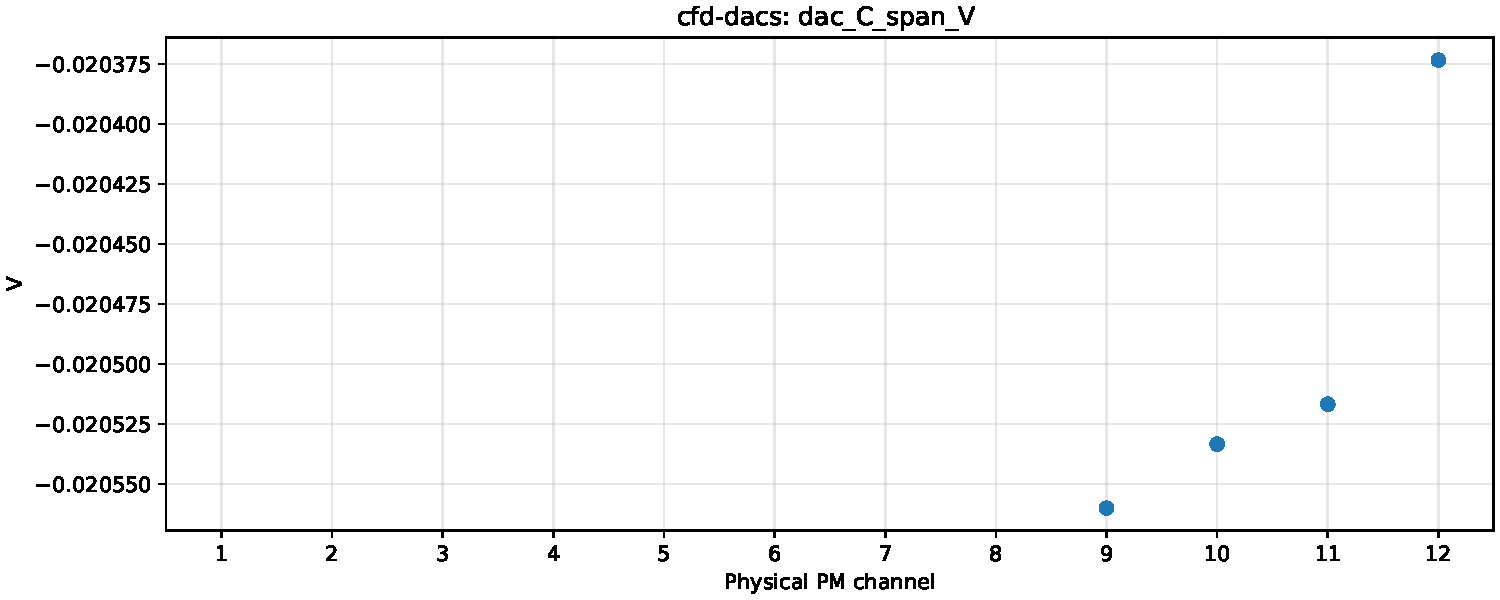
\includegraphics[width=\textwidth]{figures/figure-037.pdf}\end{center}
\begin{center}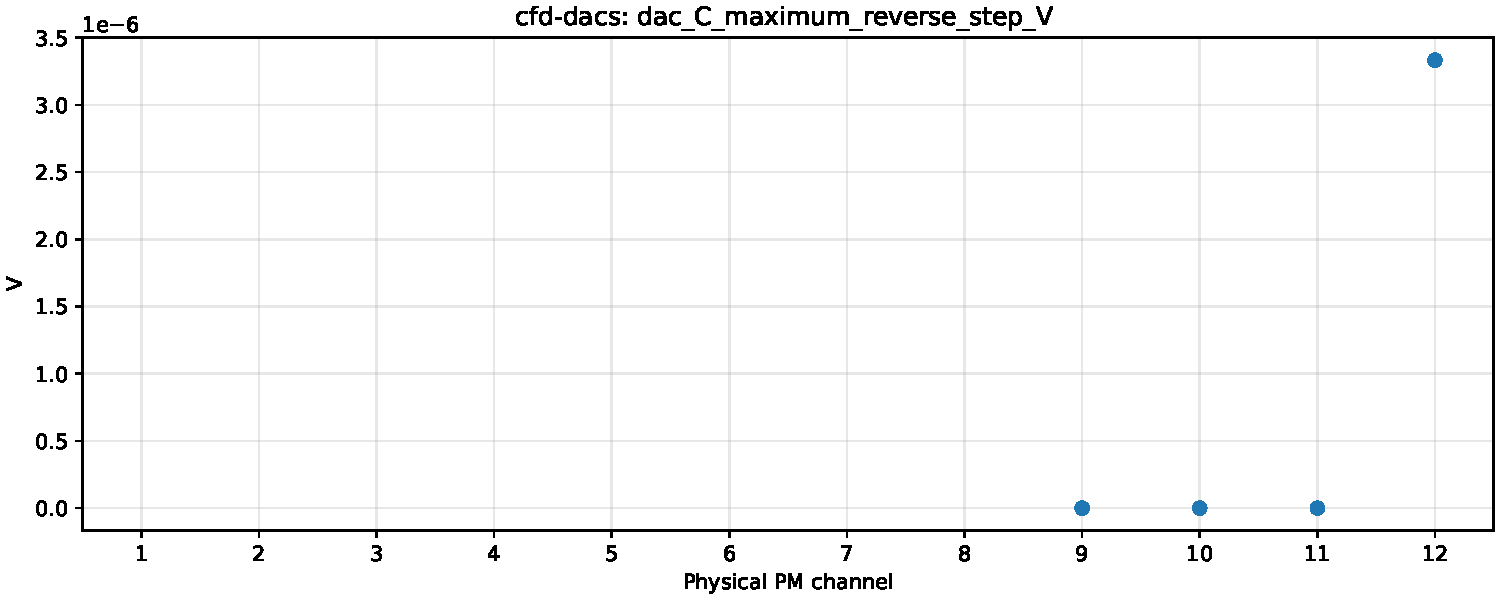
\includegraphics[width=\textwidth]{figures/figure-038.pdf}\end{center}
\begin{center}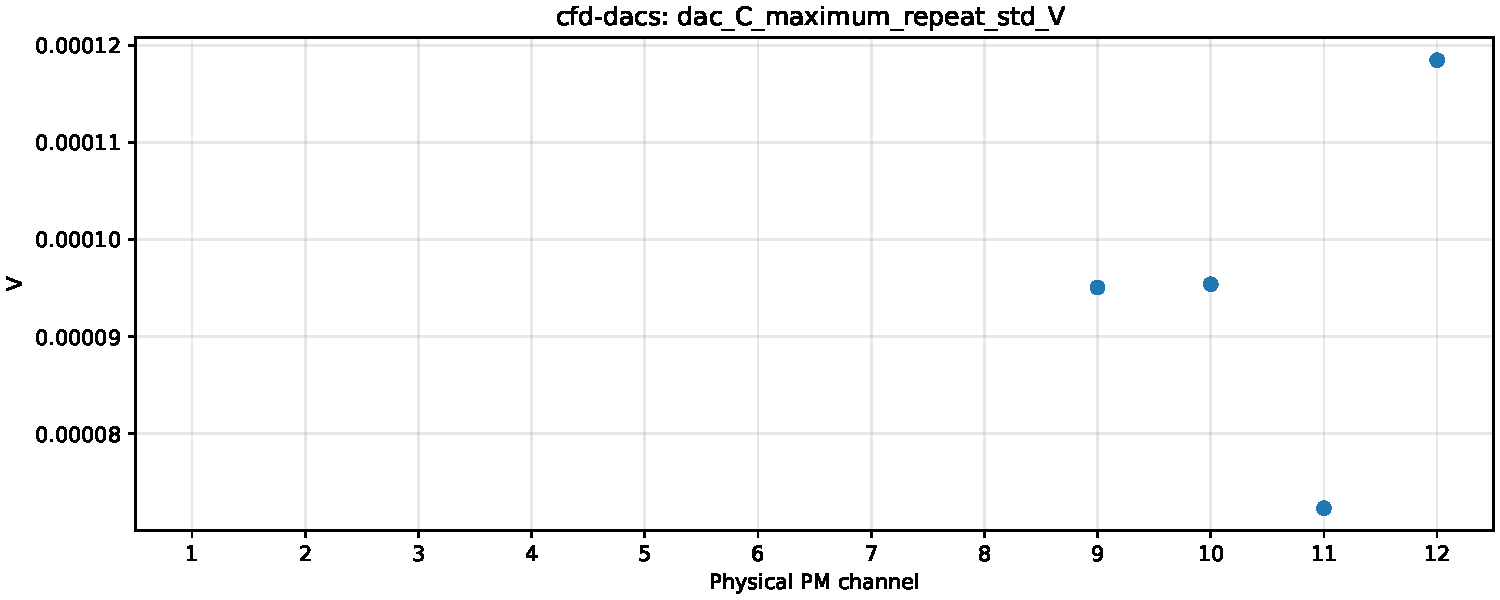
\includegraphics[width=\textwidth]{figures/figure-039.pdf}\end{center}
\begin{center}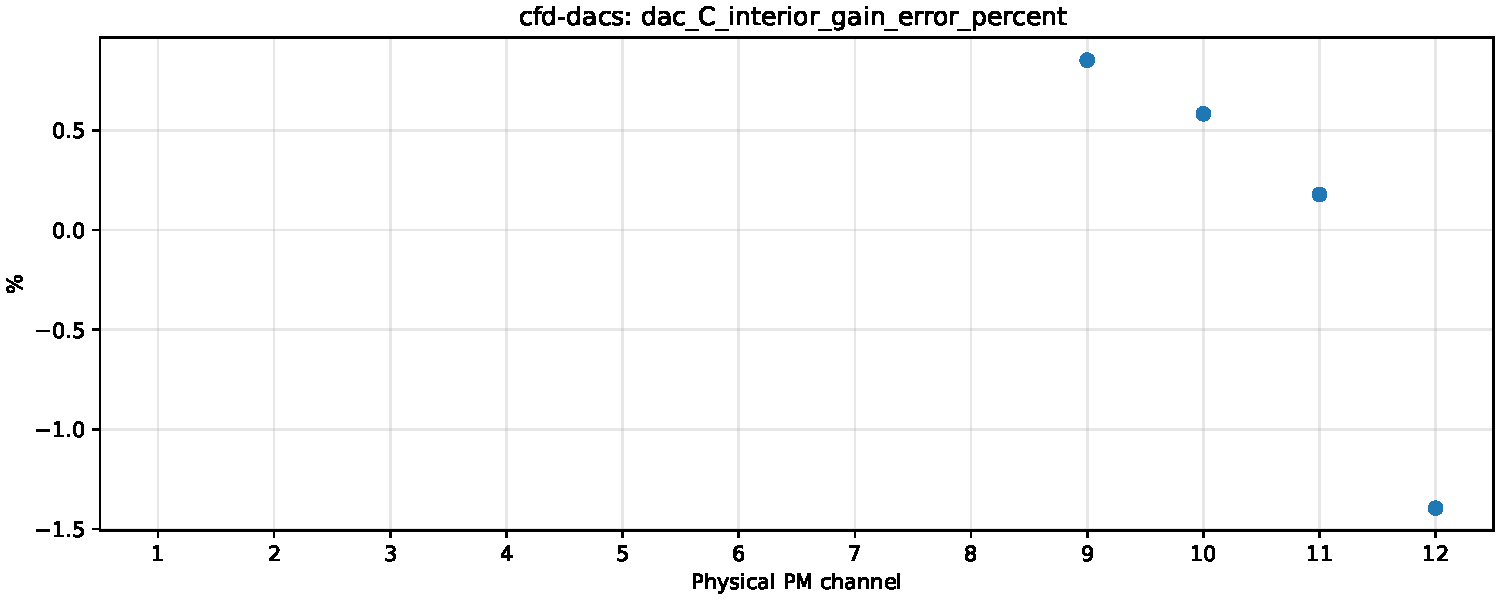
\includegraphics[width=\textwidth]{figures/figure-040.pdf}\end{center}
\begin{center}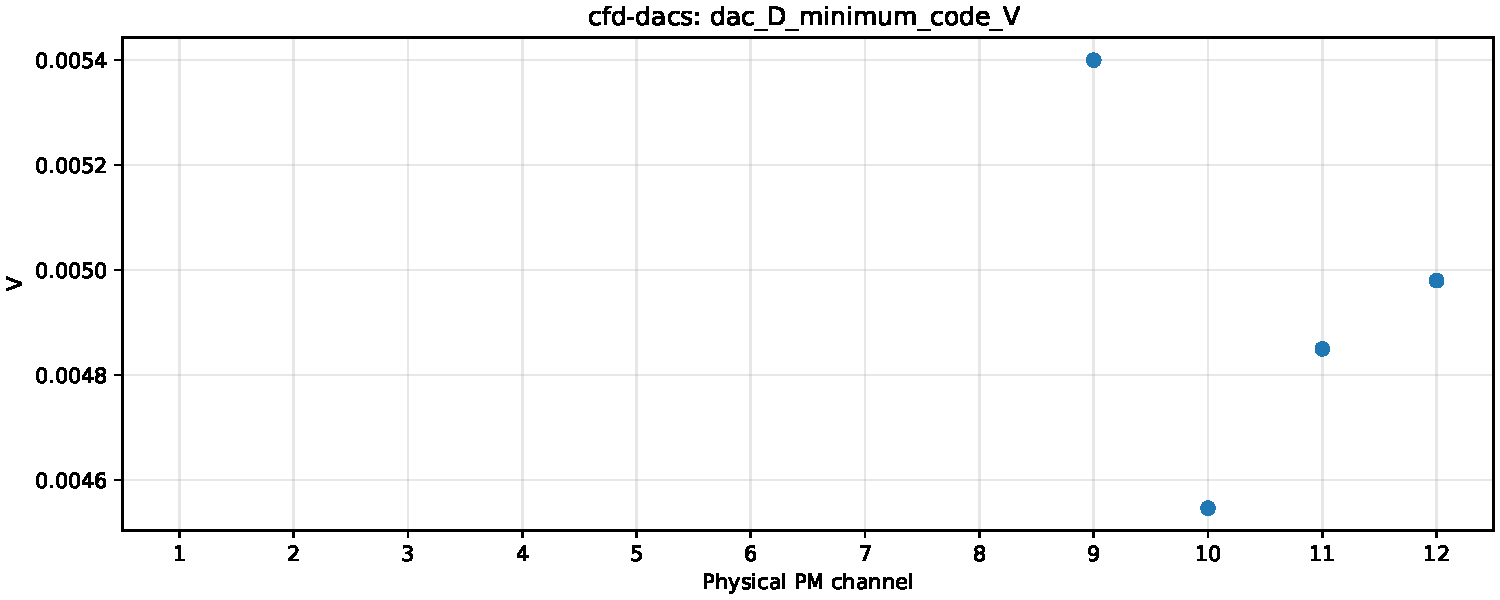
\includegraphics[width=\textwidth]{figures/figure-041.pdf}\end{center}
\begin{center}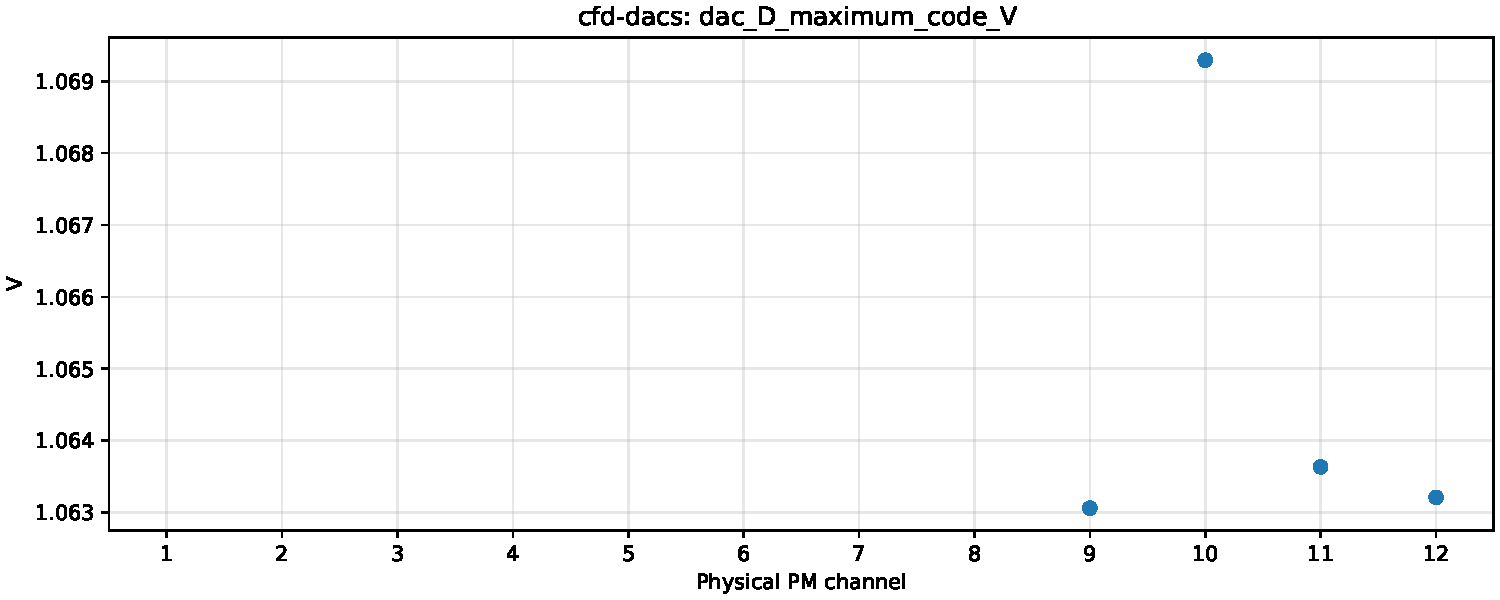
\includegraphics[width=\textwidth]{figures/figure-042.pdf}\end{center}
\begin{center}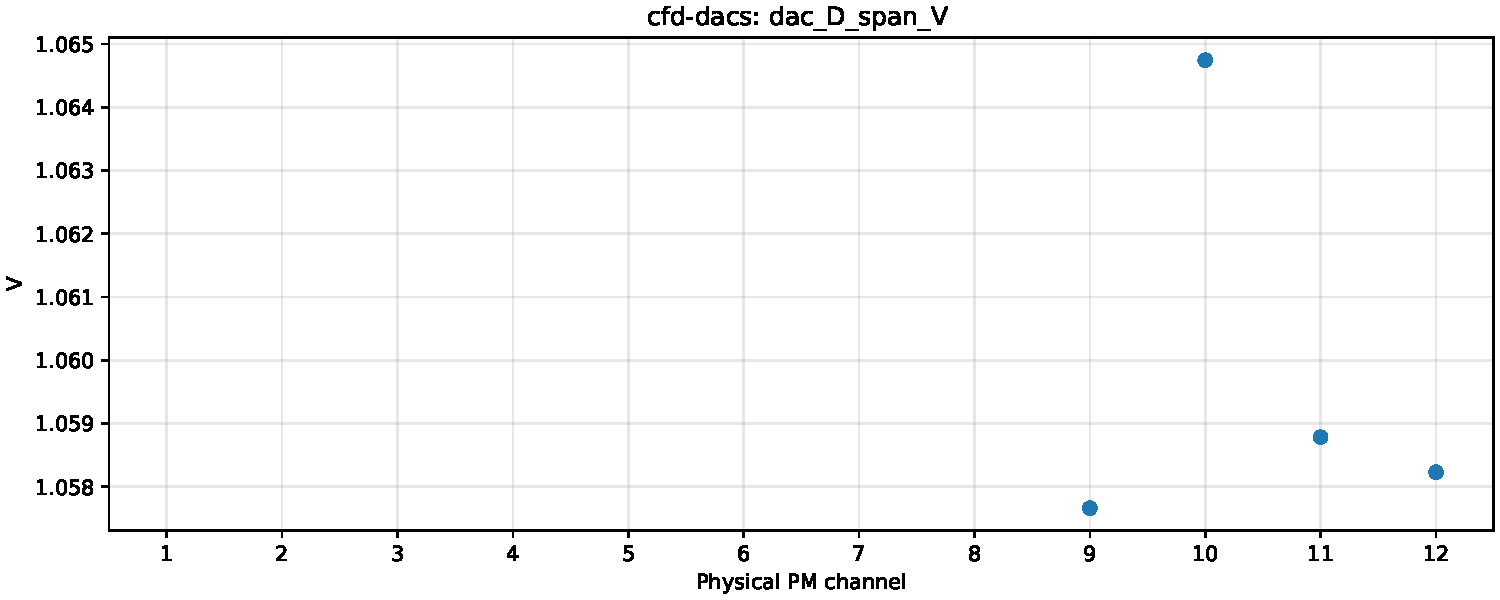
\includegraphics[width=\textwidth]{figures/figure-043.pdf}\end{center}
\begin{center}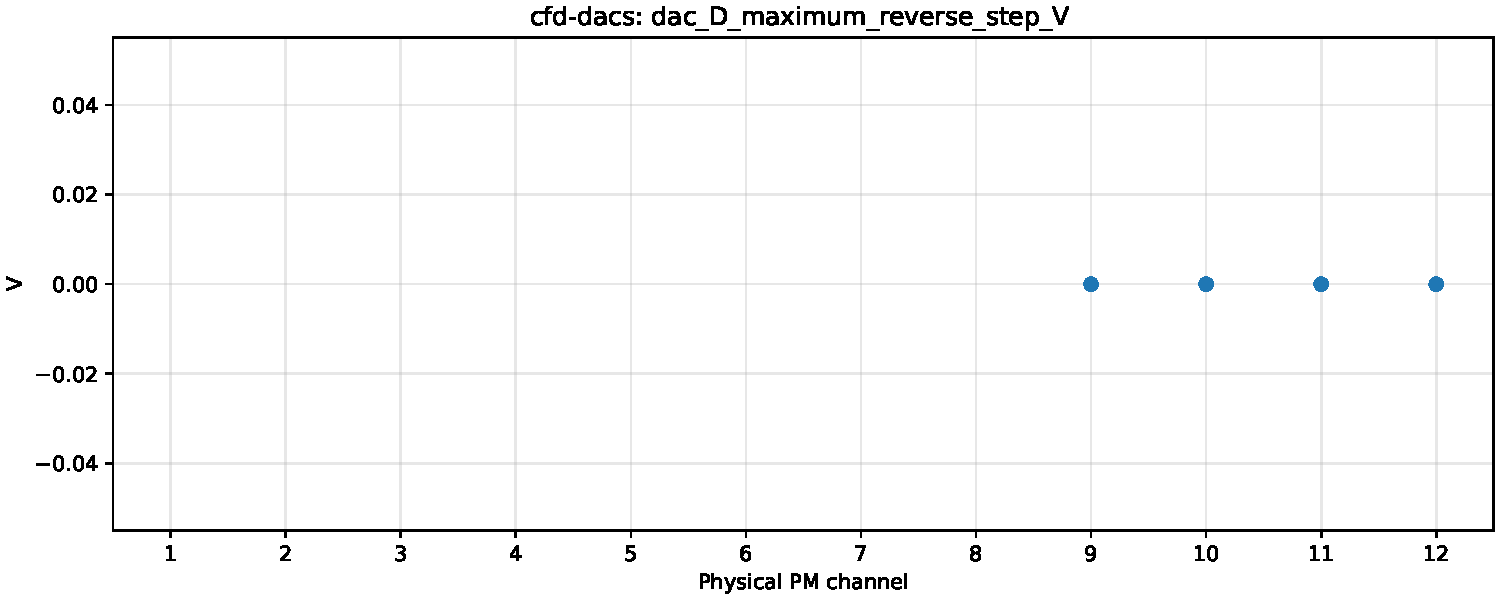
\includegraphics[width=\textwidth]{figures/figure-044.pdf}\end{center}
\begin{center}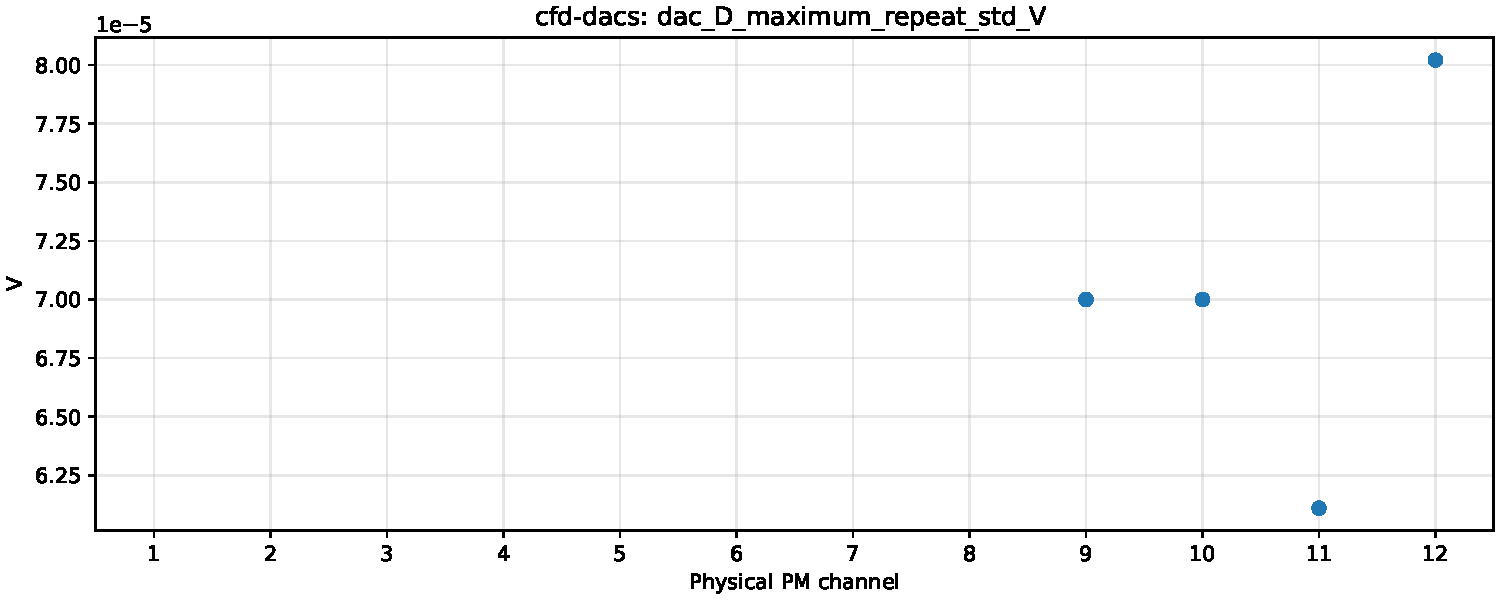
\includegraphics[width=\textwidth]{figures/figure-045.pdf}\end{center}
\begin{center}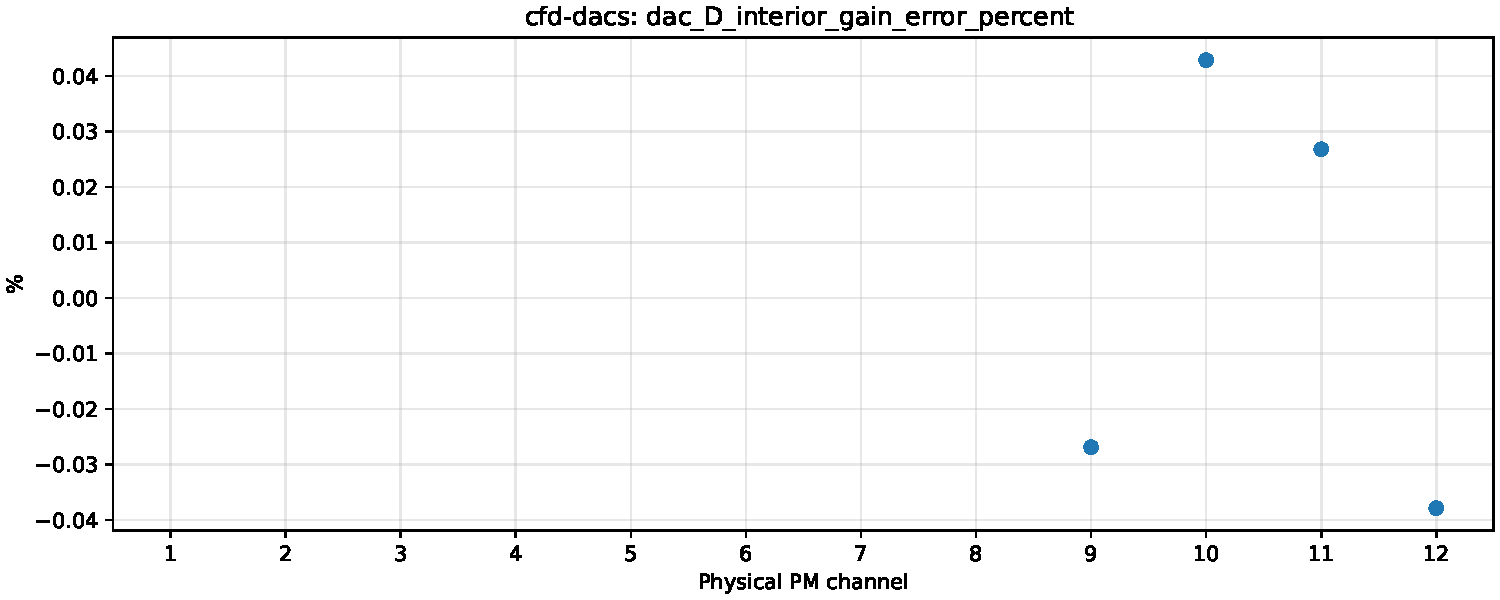
\includegraphics[width=\textwidth]{figures/figure-046.pdf}\end{center}
